\documentclass[twoside, 11pt, openright]{report}

\usepackage[utf8]{inputenc}
\usepackage{hyperref}

\usepackage{verbatim}
\usepackage{graphicx}
\usepackage{epstopdf}
\usepackage{listings}
\usepackage{calc}

\lstdefinelanguage{CPNML}
{
	morekeywords={colset,var,val,fun,let,in,end},
	morekeywords={union,bool,string,int,unit,enum,index},
	morekeywords={list,record,product,subset,alias},
	sensitive=true,
	morecomment=[s]{(*}{*)},
	morestring=[b]",
	basicstyle=\ttfamily,
	breaklines=true,
	frame=lines
}
\lstMakeShortInline{|}


\newcommand{\clearemptydoublepage}{\newpage{\pagestyle{empty}\cleardoublepage}}

\newcommand{\com}[1]{
        \mbox{}
       \marginpar{\hrule\footnotesize\raggedright\hspace{0pt}#1\vspace{2mm}}}

\newcommand{\fig}[4][0.5]{
	\begin{figure}
	\centering
	\includegraphics[scale=#1]{figures/#2}
	\caption{#3}
	\label{fig:#4}
	\end{figure}
}
\newcommand{\figrot}[4][0.5]{
	\begin{figure}
	\centering
	\includegraphics[scale=#1,angle=90]{figures/#2}
	\caption{#3}
	\label{fig:#4}
	\end{figure}
}
\newcommand{\figref}[1]{Fig.~\ref{fig:#1}}
\newcommand{\lstref}[1]{Listing~\ref{lst:#1}}

\begin{document}
\lstset{language=CPNML,tabsize=1,basicstyle=\ttfamily\footnotesize}

\begin{comment}

\pagestyle{empty}
\pagenumbering{roman}

\vspace*{\fill}
\begin{flushright}
  {\Huge\sf Design and Evaluation of a}\\[2ex]
  {\Huge\sf Framework for Annotating}\\[2ex]
  {\Huge\sf Coloured Petri Net Models}\\[2ex]
  {\Huge\sf with Code Generation Pragmatics}\\[4ex]
  {\huge\sf Mikal Hitsøy Henriksen} 
\end{flushright}
\noindent\rule{\linewidth}{1mm}\\[-.5ex]
\noindent\rule{\linewidth}{2.5mm}
\vfill
\begin{center}
  {\huge\sf Master's Thesis}\\[\fill]
%  
\includegraphics{au-segl.ps}\\[\fill]
  {\sf Department of Computer Engineering\\Bergen University College\\Norway}
\end{center}
\begin{center}
  {\sf \makeatletter\@date\makeatother\\Supervisor\\Lars Michael Kristensen}
\end{center}
\vspace*{\fill}
\clearemptydoublepage


\begin{abstract}
Model Driven Engineering (MDE) is a software development methodology that
relies  on developing domain models that represent knowledge concepts and
activities that belong to the application domain. When applied in software development, MDE aims
to support automatic generation of source code from the domain models, which
also provides a means for keeping design models and implementation synchronised.

One of the modeling languages that can be used in MDE is Colored Petri Nets
(CPN). It is a type of high-level Petri Net, suited for describing,
analysing and validating systems that consist of communication, synchronisation,
and resource sharing between concurrently executing components. A CPN model can
accurately model many types of software systems, but cannot directly be used
to generate a software implementation. Research is being conducted to develop an
approach for annotating CPN models of communication protocols to enable source
code generation.

This thesis has resulted in a prototype application for annotating CPN models
with code generation pragmatics. The prototype builds on the ePNK framework,
which uses the Eclipse Modeling Framework (EMF) to provide an extensible
platform for working with CPN models.
The prototype is desgned as a plugin for Eclipse. It can import
models created by CPN Tools and lets the user annotate the models with code
generation pragmatics. The prototype has been evaluated by applying it to a set
of protocol CPN models. We show that CPN models annotated with code generation
pragmatics are a viable method for use in model-driven development of protocol
software.
We also give a detailed case study of modeling the WebSocket protocol, including
verification and analysis of the CPN model using state space exploration, and
annotation with code generation pramatics.

\end{abstract}

\clearpage
\tableofcontents
\clearemptydoublepage



\pagestyle{headings}
\pagenumbering{arabic}
\setcounter{page}{1}

\end{comment}
%\chapter{Introduction}
\label{chap:introduction}

%Zooming in part of the introduction
Software development is a notoriously error-prone process, and writing a program of a certain size without errors is infeasible. A major part of software development is therefore concerned with finding bugs and eliminating them. Testing is widely used as a technique to detect bugs, but the programmer never knows whether the absence of failed test cases means a missing test case, or that the software is free of errors. Writing an appropriate set of test cases can be very challenging, and running them can be a time-consuming process. It is especially difficult to write exhaustive test cases for concurrent systems, e.g., for a communication protocol where several process instances are executing at the same time.

Building an abstract representation of the system in form of a \emph{model} is another way to detect bugs. The model can be used to verify properties in a system, e.g., that a system does not contain any deadlocks, or that a communication protocol behaves correct in an unreliable network. In Fig.~\ref{fig:specmodelimpl} we show a typical way of using models in software development. The model is build on the basis of a system specification written in plain English. After verifying that the model has the desired properties, it can be used as a basis of an implementation. 

\begin{figure}[h!]
\centering
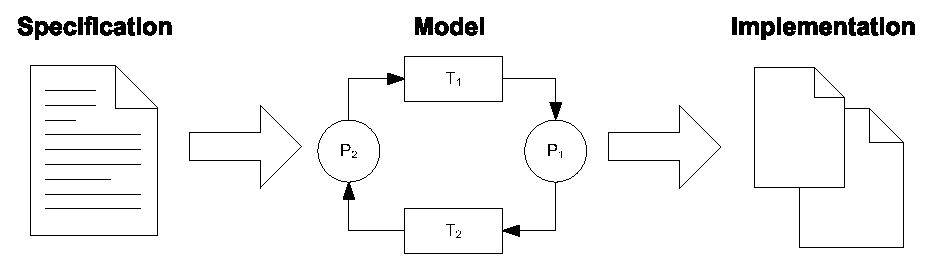
\includegraphics[scale=0.7]{introduction/graphics/spec_model_impl_figure.eps}
\caption{Phases in software development using models}
\label{fig:specmodelimpl}
\end{figure}

%Formal verification advantages
The advantage of constructing a model in the development phase is at least threefold: 
\begin{itemize}
\item Developers are forced to be precise about essential parts of the specification in the process of building the model. Specifications are often ambiguous because they are written in plain English, and details may be missing in the specification. Finding these errors early in the development process can save a lot of resources later.

\item By using the appropriate tools it is possible to perform simulations of a model. A simulation is very similar to an execution of a program. It shows how the model behaves in different situations which can be used to debug the specification. 

\item From a model it is possible to generate a state space, which is a directed graph, where states are represented as nodes and events \ignore{, that changes the system to a new state, }are represented as arcs. The state space can be explored in order to mathematically prove that the system has a given property. This is important in systems were an error can have catastrophic consequences, e.g., in the software controlling the cooling system of a reactive core in a nuclear power plant. 
\end{itemize}

% State space analysis disadvantages
A problem with state space analysis is that the number of states a system can reach often grow rapidly when the model becomes more complex. This is known as the \emph{state explosion problem} \cite{Val98}, and is a big challenge when performing state space exploration. It is often possible to restrict the model, or build the state space partially and still find errors in the system. 

% Translating the model to code
Another problem with the approach shown in Fig.~\ref{fig:specmodelimpl} is that there may be a mismatch between the specification, the model, and the actual implementation. This is because the translation: specification $\rightarrow$ model $\rightarrow$ imhhhplementation is done manually, and hence errors may be introduced in each step of the translation. A way to reduce this problem is to use the model as the specification and automatically generate the implementation from the model. The details abstracted away in the model will of course also lack in the implementation, but eliminating errors in the important parts of the system would lead to more reliable software with fewer errors. \ignore{and could save a lot of resources compared to making the translation manually.}\\

% Example to motivate automatic code generation
Network protocols are an example of why automatic code generation is useful in software development. The \underline{Dy}namic \underline{M}ANET \underline{O}n-demand (DYMO) Routing Protocol \cite{refWorks:69} is a protocol for routing in mobile ad-hoc networks. The Internet Draft describing the protocol is currently at version 16 and about to become an Internet Standard. The specification is written in English describing the different operations of the protocol, and it can be used as a basis for an implementation. Because natural language specifications are often ambiguous translating them to either an implementation or a model requires that the developer make some choices. These choices can make the implementation flawed, and it can also make interoperability between different implementation difficult. 

Specifying DYMO as a formal model (instead of plain English) would exclude ambiguities in the specification. It would also make it easier to directly find errors or verify properties of the specification. In an earlier project \cite{RefWorks:6} we showed, that a model of the DYMO protocol containing all the mandatory parts can be constructed using relatively few resources. The problem is that manually implementing the protocol based on the model may introduce errors, and it would therefore be better \ignore{and more cost-efficient} to generate most of the implementation automatically. In the case of the DYMO protocol, technical details like packet formats and configurations are abstracted away in the model, so they would have to be implemented manually. But the protocol logic and the structure of the implementation would be generated automatically and therefore preserving the behaviour of model in the code.


\section{Coloured Petri Nets}

Petri nets \cite{Petri} is an executable graphical modelling language represented by a bi-graph consisting of nodes and arcs. It can be used to describe a discrete-event concurrent system. An example of such a concurrent system could be a communication protocol. A model could be used to analyse whether it is possible to bring the protocol in an undesirable state, e.g., a deadlock. Nodes in a Petri net are either transitions representing discrete events, or places representing conditions. Arcs in a Petri net describe the pre- and post-condition relation between transitions. 

% Coloured Petri Nets
Coloured Petri Nets (CP-nets or CPNs) \cite{RefWorks:3} is a high-level Petri net language, i.e., the Petri net formalism with added high-level programming functionalities. The programming language used is CPN ML which is based on the general-purpose functional programming language Standard ML \cite{RefWorks:67}. CPN ML provides support for commonly used functionality, e.g., defining data types and manipulating data. Every part of the CPN language has a formal definition, i.e., it is defined mathematically what will happen, e.g., when events occur in the model. This makes it possible to simulate an execution of a CPN model to inspect which states the model can reach. 

CPN Tools \cite{RefWorks:3} is a graphical CPN editor in which it is possible to construct and simulate CPN models. Through the graphical user interface the user can construct a model and do step-by-step simulation. This is much easier than constructing and simulating the CPN model according to the mathematical definition by hand.

When performing a simulation of a model, only one possible execution of the system is explored. But often it is interesting to look at every possible execution of the system to analysis whether it is possible for the model to reach an undesirable state. As mentioned, this can be done by generating and exploring the state space of the model to analyse the behaviour of the system. There exist a range of tools that suppot state space exploration. CPN Tools has built-in support for generating and exploring state spaces. Another computer tool is the \underline{A}SCoVeCo \underline{S}tate space \underline{A}nalysis \underline{P}latform (ASAP) \cite{RefWorks:92}. ASAP is a platform that supports state space analysis of CPN models using state-of-the-art exploration algorithms. The program is built on top of the Eclipse Rich Client platform \cite{RefWorks:73} which makes is very easy to extend, a fact we take advantage of later in this thesis.

\section{Code Generation}
An often used definition of code generation is one computer program producing another computer program in an automatic way. A well known type of code generator is a compiler, e.g., Sun's javac \cite{refWorks:70} or GNU's GCC \cite{refWorks:71}. A compiler typically takes a human-readable text file as input and outputs an executable program. The produced program is often low-level code, e.g., machine code.

The type of code generation presented in this thesis is \emph{source code generation}. The input to this kind of code generator is a formal model specified for instance in a graphical modelling language, and the output is human-readable source code written in a high-level programming language. A compiler has the advantage that high-level programming languages are designed such that the translation into low-level code always makes sense and has equivalent behaviour. Source code generation from a formal model do not have the same advantage. A model is an abstraction of a system and because of the generality of the model it is often very hard to obtain equivalent behaviour in the source code.

Also, the level of abstraction has to be taken into consideration. In one model the focus might be on the details of packet transmission in a network, whereas in another model these details might have been abstracted away. This can make it hard to generate code since it is difficult to make an interpretation of the structures in the model.

\section{Thesis Aims and Results}
The aim of this thesis is to develop a technique to automatically generate code from CPN models. The code should be readable and intuitive such that the user can read, modify and extend the generated code. We also require that the model should be clearly recognizable in the generated code since the people working with the generated code would typically be very familiar with the model. The technique should allow different target languages to be used, e.g., C, Java, SML or Erlang. However the target language should be invisible in the model and the usual inscription language should be used in the model.

We achieved the aim by defining a subclass of CP-nets called Process-Partitioned CP-nets (ProPCP-nets or ProPCPNs). ProPCPN models preserve most of the general-purpose strength of CP-nets as we show by constructing a model of the advanced DYMO protocol. We have developed a technique that translates from the class of ProPCP-nets to the Erlang programming language, and created an implementation of the technique as a proof of concept. The implementation is able to generate readable code from the DYMO model, and we validate that the generated code has the same behaviour as the model. 


\ignore{
%% OLD AIM:
%% Model: Restriction vs. expressiveness, target language invisible
Our aim is to define a subclass of CP-nets which preserves the general-purpose strength of CP-nets, but enables us to generate code for the models in the class. To show the expressive power of the class we construct a model of the complex communication protocol DYMO in this class. Our focus in the translation is more on generating readable code than on generating high performance code. It is for instance more important that the programmer is able to recognize the model in the code than making the code highly optimised.

%% Tool
As a proof of concept we implement a tool which given a CPN model in our subclass of CPNs generates an Erlang source code implementation of the model. The implementation should have the same behaviour and properties as the model.

}

\section{Thesis Outline}
The structure of the thesis is described below. The thesis is written in close cooperation between the two authors, but as required we have divided the responsibility of the chapters. 

\begin{description}
\item[Chapter~\ref{chap:background}~\nameref{chap:background}] In this chapter we establish the background for understanding the thesis. We present the CPN model of a producer-consumer system which is the running example throughout the thesis. We also present the target language of the translation, namely Erlang, and describe the basic constructs of the Erlang language. Kristian is responsible for Sec.~\ref{sec:cpn}, and Mads is responsible for Sec.~\ref{sec:erlang}. 

\item[Chapter~\ref{chap:codegeneration}~\nameref{chap:codegeneration}] Different approaches to code generation is discussed on the basis of related work. We illustrate some of the approaches using manually translated code examples, and discuss advantages and disadvantages. Mads is responsible for this chapter.

\item[Chapter~\ref{chap:netclass}~\nameref{chap:netclass}] ProPCPN is a subclass of CPN that we constructed to generate code from, and we give an intuitive description as well as a formal definition of the net class. We also show that the producer-consumer model presented in chapter~\ref{chap:background} fits into this subclass. Mads is responsible for this chapter.

\item[Chapter~\ref{chap:translation}~\nameref{chap:translation}] In this chapter we present a technique to generate Erlang source code from ProPCPN models. We present all the phases of the translation, and use the simple producer-consumer model to illustrate the translation. Mads is responsible Sec.~\ref{sec:cpntodcpn}, Sec.~\ref{sec:dcpntocfg}, and Sec.~\ref{sec:cfgtoast}. Kristian is responsible for Sec.~\ref{sec:astest}, Sec.~\ref{sec:esttocode}, and Sec.~\ref{sec:advancedissues}.

\item[Chapter~\ref{chap:tool}~\nameref{chap:tool}] In this chapter we present our implementation of the translation technique presented in chapter~\ref{chap:translation}. We also validate the code generated from the producer-consumer model. Kristian is responsible for this chapter.

\item[Chapter~\ref{chap:dymo}~\nameref{chap:dymo}] In this chapter we show the expressive power of ProPCPN models by constructing a model of the industrial-sized protocol DYMO. We automatically generate code from the model using our implementation of the translation, and show that the protocol logic from the model is preserved in the generated code. Kristian is responsible for this chapter.

\item[Chapter~\ref{chap:confutwo}~\nameref{chap:confutwo}] Finally, we conclude and summaries on the findings in this thesis and outline some directions for future work.

\end{description}

The implementation of the translation can be found on the enclosed CD-ROM (see appendix \ref{appsec:cd} for more information). The reader is expected to have a basic understanding of formal models, whereas the formal modelling language Coloured Petri Nets is introduced in section \ref{sec:cpn}. Knowledge about SML (or a similar functional language) is also expected, whereas the fundamental concepts of the functional programming language Erlang are explained in section~\ref{sec:erlang}.

%\chapter{Background}\com{Bør kanskje gjenvurdere om det skal hete
``Background''}
\label{chap:background}

\section{The WebSocket Protocol}
The primary case study for this thesis is the WebSocket protocol 
\cite{draft-ietf-hybi-thewebsocketprotocol}. From the abstract of the document:
\begin{quote}The WebSocket protocol enables two-way communication between a
client running untrusted code running in a controlled environment to a
remote host that has opted-in to communications from that code.
\end{quote}

\fig[0.4]{WebSocketSequenceDiagram.pdf}{Sequence Diagram of the WebSocket
protocol}{wssequence}

\figref{wssequence} shows the basic sequence of the WebSocket protocol. To
establish a connection, a client sends a specially formatted HTTP request to a
server, which replies with a HTTP response. Once the connection is
established, the client and server can then freely send WebSocket message
frames, until either endpoint sends a control frame with the opcode 0x8 for
close and optionally data about the reason for closing. The other endpoint then
replies with the same opcode and data, and the connection is considered closed.

From the RFC document:

\begin{quote}
	Conceptually, WebSocket is really just a layer on top of TCP that
	does the following:
	\begin{itemize}
		\item adds a Web "origin"-based security model for browsers
	
		\item adds an addressing and protocol naming mechanism to support
		multiple services on one port and multiple host names on one IP
		address;
	
		\item layers a framing mechanism on top of TCP to get back to the IP
		packet mechanism that TCP is built on, but without length limits
	
		\item includes an additional closing handshake in-band that is designed
		to work in the presence of proxies and other intermediaries
	\end{itemize}
\end{quote}

\section{Coloured Petri Nets}

Common usage: Process and protocol modeling, concurrent programming. Operations:
Simulation, verification and analysis. More recently also software design.

The structure of CPN models will be explained gradually through the case study 

\subsection{CPN Tools}

Graphical tool used to design CPN models. 

\begin{comment}

\subsection{CPN ML}
	


		
		The simple types available are unit, boolean, integer, string, enumerated
		and index. A unit can have one value: \lstinline:():. Enumerated colour sets
		can have specified values, while index colour sets define an indexed range of
		values. 
		
		The compound types are:
		\begin{description}
		\item[Product] A combination of colour sets separated by \lstinline:*:. The
		postal code and city example from earlier would be
		\lstinline:product INT*STRING:, and a colour would be (5055,''Bergen'');
		\item[List] A list of items that belong to the same colour set.
		\item[Record] Similar to a product, but each element is named. The postal code
		and city example would give \lstinline-record Code:INT*City:STRING- and a
		colour would be \lstinline:{Code=5055,City="Bergen"}:
		\item[Union] This is used if a place should be able to contain colours from
		different colour sets, or if such colours should be handled in the same way at a
		point in the model. They can also contain simple identifiers, like an
		enumeration. An example is shown in Listing \ref{lst:overview_colset}.
		\end{description}
		
		For full syntax definition, please refer to the CPN Tools
		documentation. (ref?)

\end{comment}
\section{The WebSocket CPN Model}

The websocket protocol is the primary case study of this thesis. 
In this section the model that has been built is described in full detail.

\subsection{Overview}

	\fig{Overview.eps}{Overview of CPN model of the WebSocket protocol}{overview}
	
	\figref{overview} shows the top-level Overview module of the WebSocket
	CPN model.
	
	The model has been laid out to resemble part of the OSI model \cite{osi7}, where
	Client Application and Server Application each correspond to the top two
	layers Application and Presentation, Client WebSocket and Server WebSocket
	correspond to the Session layer, and Connection corresponds to the lower layers
	Transport, Network, Data Link and Physical.
	
	\subsubsection{Model basics}
	A Petri Net model consist of pages, or modules, that contain Places,
	Transitions and Arcs.
	
	Places are represented by circles. They can contain colours from a specified
	colour set, and have markings to define initial colour(s).  As an example, in
	the lower right we have the Server Send place. This place can have
	\lstinline:PACKETLIST: color tokens, and has an initial marking of an empty
	list \lstinline:[]:. It currently has one colour shown in the green box,
	\lstinline:1`[]:, which means one of an empty list. The number in the circle
	shows the total number of colours in this place.
	
	A colour can mean a single value like the integer 3, the string ``Hello'' or
	simple units which resemble Tokens from regular Petri Nets. A colour set is a
	set of such colours, for example all integers, the integers from 1 to 100, all
	lowercase letters, or all strings of length 5. These are examples of simple
	colour sets, as they each consist of basic data types. Compound colour sets are
	made by combining the simple ones in different ways to create data structures, for
	example an integer together with a string might describe a postal code and
	city. This will be described in more detail in the next section.
	
	Transitions are represented by rectangles. 
	
	Double-bordered rectangles represent substitution transitions which are bound
	to sub-modules. These are separate modules that have input and output places
	that connect to the places on their parent module. This enables us to keep
	the model structured and readable, and also allows reuse of modules in
	different parts of the model by instancing them, which will be described toward
	the end of the chapter. The details of each submodule is described in the
	following subsections.
	
	Arcs are directed arrows going between a place and a transition.
	
	The State of the model is defined by the current colors in
	each place. A Transition can consume colors from places if there is an arc from
	the place to the transition, and produce new colors in places where there is an
	arc from the transition to the place. This changes the state of the system.
	
	
	\subsubsection{Declarations}
	
	CPN Tools uses the CPN ML language to specify declarations and net inscriptions.
	This language is an extension of the functional programming language Standard
	ML, developed at Edinburgh University.
	
	All coloursets, variables, symbolic constants and functions have to be declared
	before they are used in the model. In CPN Tools these declarations can be
	grouped together, but they are still parsed sequentially, so if one declaration
	depends on another, it has to be declared after its dependency.

	Colour sets are defined with the following syntax:
	
	\lstinline:colset name = <type-specific>;:
	
	Names are always capitalised in this thesis, but any CPN ML identifier is
	valid.
	
	The places in the Overview use the following colour set definitions:
	
	\begin{lstlisting}[label=lst:overview_colset,caption=Overview colour
	sets,gobble=1]
	colset OPERATION = with CONNECT | TEXT | BINARY | PING | PONG | CLOSE;
		
	colset MESSAGE = record Op: OPERATION *	Message: STRING;
	
	colset MESSAGES = list MESSAGE;
	
	colset CONN_RESULT = bool with (fail, success);
	
	colset EVENT = union Msg:MESSAGE + ConnRequest + ConnResult:CONN_RESULT;
	
	colset EVENTS = list EVENT;
	
	colset CONN_REPLY = bool with (reject, accept);
	
	colset MSG_OR_CONN_REPLY = union Msg':MESSAGE + ConnReply:CONN_REPLY;
	
	colset MSGS_OR_CONN_REPLY = list MSG_OR_CONN_REPLY;
	
	colset PACKET = union HttpReq:HTTPREQ + HttpRes:HTTPRES + WsFrame:WSFRAME;
	
	colset PACKETLIST = list PACKET;
	\end{lstlisting}
	
	The \lstinline:OPERATION: colour set is an enumeration that represents the
	different types of messages that can be passed between the application and the
	protocol layer. All of these correspond with opcodes
	used in WebSocket frames, except \lstinline:CONNECT: which is used for
	initiating a connection.
	
	A \lstinline:MESSAGE: is a record that consists of an
	\lstinline:OPERATION: and the \lstinline:STRING: message body. Both
	data- and control-frames can have messages, although control-frame
	messages might not be shown to the user. Colours from record color sets can
	have their component colors referenced by name, in this case \lstinline:Op: and \lstinline:Message:. We can also have a list of \lstinline:MESSAGES: to keep them ordered. Lists will be explained in detail
	later where they are used and manipulated in the model.
	
	The WebSocket layer also needs a way to notify the application about connection
	results, which is done with the \lstinline:EVENT: color set. This is a union
	color set which can be either a \lstinline:MESSAGE:, a \lstinline:ConnRequest:
	identifier (with no other color associated), or a \lstinline:CONN_RESULT:. A
	union color set is used if a place should be able to contain colours from
	different colour sets, or if such colours should be handled in the same way at
	a point in the model. They can also contain simple identifiers (like
	\lstinline:ConnRequest:). And like \lstinline:MESSAGES: we can have a list of
	\lstinline:EVENTS.:
	
	The client application sends \lstinline:MESSAGES: to the WebSocket layer and
	receives \lstinline:EVENTS: back. The server application also receives
	\lstinline:EVENTS:, but can send either a \lstinline:MESSAGE: or a
	\lstinline:CONN_REPLY:, which is used for connection attempts. The
	\lstinline:CONN_REPLY: colourset is simply a boolean value with different
	names for true and false, for improving readability and semantics. A union of
	these two types must exist, \lstinline:MSG_OR_CONN_REPLY:, so the same place
	can be reused.
	
	TODO: Noe om hvorfor vi bruker kun en plass for dette
	
	Both the client and server WebSocket layers send and receive
	\lstinline:PACKET: colors, a union of three types of data. \lstinline:PACKET:s
	are abstract and not fully modeled actual network packets, as this is not
	relevant to how WebSocket works. Ther list version \lstinline:PACKETLIST: These
	color sets are described in the section for the Connection module.

\subsection{Client Application}

	\fig[0.4]{ClientApplication.eps}{The Client Application}{client_app}
	
	This module (\figref{client_app}) is laid out from top to bottom to loosely show
	the sequence of operation, as is most of the other modules.
	
	The places at the bottom represent the interface to the WebSocket layer. To
	simplify the overview model and facilitate easier later modification
	and expansion, we have only two places that act as input and output. These are
	called Receive Client Events and Send Client Message, and are tagged In and
	Out respectively. These are connected to the respective places on the
	Overview, which are also connected to corresponding places in the WebSocket
	Library.
	
	
	\subsubsection{Variables}
	
		The arcs here have inscriptions on them containing variables. Variables are
		declared globally and can only be bound to colours of the colourset they are
		defined for. 
		
		When a transition fires, it will bind the tokens it is consuming to the
		variables of the inscriptions on the arcs from the respective places. These
		variables can then be used to produce new tokens, by direct manipulation
		and/or in conditional statemens. The expression that will produce the desired
		result is inscribed on the output arc. 
		
		A set of variables has been declared for the simple coloursets as follows:
		
		\begin{lstlisting}[label=lst:standard_vars,caption=Simple Colourset Variables]
		var u, u1, u2, u3: UNIT;
		var b, b1, b2, b3: BOOL;
		var i, j, k: INT;
		var s, s1, s2, s3: STRING;
		var ss, ss1, ss2: STRINGLIST;
		\end{lstlisting}
		
		Several variables for the same coloursets have been created for convenience in
		the cases where colours of the same type is consumed from different places. If the same variable was
		used on each arc from two different places, both places would need a token
		with the same value. 
		
		Variable declarations will be listed as they are encountered in the model.
		As a general guideline, most variables are named with the first letter of its
		colourset for non-lists, and the same letter plus the letter s for lists. On
		this submodule we have the following variables:
		
		\begin{lstlisting}[label=lst:client_app_vars,caption=Client Application
		Variables]
		var msg: MESSAGE;
		var msgs, msgs2: MESSAGES;
		var es: EVENTS;
		\end{lstlisting}
	
	\subsubsection{Queues}
	
		A lot of the places in this model rely on tokens being consumed in the same
		order they are produced, and to enforce this, queues are used, facilitated
		by list colour sets. To describe a list in SML, we use square
		brackets \lstinline:[ ]:. By themselves they represent an empty list. To describe a populated list, we
		write each token inside the brackets separated by commas. An example of this
		is seen in \figref{client_app} on the initial marking for the
		\lstinline:Messages to be sent: place.
		
		To process such a list, we use the \lstinline-::- operator like this:
		\lstinline-head::tail-, where head is the first element in the list, and tail
		is all the following elements. To concatenate two lists, we use the
		\lstinline:^^: operator. 
		
		To emulate the queue behaviour we need, we use a list of a colour instead of
		using the actual colour we want in that place. When we want to take an
		element from the front of the queue, we use the \lstinline-::- operator to
		bind the head and tail of the list to variables, and put only the tail back to
		the source place. When we want to append an element to a queue, we concatenate
		the queue using the \lstinline:^^: operator with a new list containing only
		the new element. To improve readability of the model, these queue operations
		have one arc slightly dimmed, to emphasise the flow direction of data.
		
		An example of this is seen in \figref{client_app} on the arc
		from the \lstinline:Send data: transition to the 
		\lstinline:Messages to be sent: place. On the left side, the list in the
		Messages to be sent place is bound to the two variables msg and msgs, and only
		msgs is put back. On the right side, we take the list in Send Client Messages
		and bind it to the variable \lstinline:msgs2:, and send back a concatenation
		of this list and a new list containing msg, which was bound earlier in the incoming arc
		from Messages to be sent. The total effect is that we take the first element
		from Messages to be sent, and add it to the end of the list in Send Client
		Message.

	\subsubsection{Program Flow}
	
		The Request connection transition at the top is highlighted by a green border,
		which means that it is enabled and ready to fire. If we were to fire this transition,
		it would consume the \lstinline:STRING: token, named s, produce a
		\lstinline:MESSAGE: token containing s, and add it to the queue in the Send
		Client Message place.
		
		Next, the Client Application waits for a \lstinline:CONN_RESULT: token, and if
		this is equal to \lstinline:success:, we add a \lstinline:UNIT: token to the
		Active Connection place. If any other messages are received before this, they
		will wait at the Receive Client Event place, since the Receive Data transition
		will not fire unless the Active Connection place has a \lstinline:UNIT: token.
		
		If and when the Active Connection place has a \lstinline:UNIT: token, the
		Client Application can start sending and receiving messages. A sample of
		messages has been predefined at the Messages to be sent place, but this would
		probably be dynamic in a real application. \com{Kanskje dette kunne vært mer
		abstrakt? Argument for hvorfor modellert på denne måten.}
		
		Finally, if the Client Application receives a \lstinline:MESSAGE: where the
		\lstinline:OPERATOR: is \lstinline:CLOSE:, nothing is put back into the Active
		Connection place, and the connection is effectively closed. 

\subsection{The Client WebSocket Module}

	\fig{ClientWebSocket.eps}{The Client WebSocket Module}{client_wslib}

	This module consists mostly of substitution transitions. The only processing
	being done directly on this module is masking of all websocket frames
	\com{Hvordan funker mask funksjonen?}, which is required from the client by the
	protocol specification.
	The rest is plumbing between the submodules.
	
	The new coloursets are for HTTP requests and responses, WebSocket frames, and
	packets. They have corresponding variables. 
	
	\begin{lstlisting}[label=lst:client_lib_colset,caption=Library colour
	sets,gobble=1]
	colset HTTP_VERB = union GET + POST + PUT + DELETE + HEAD;
	
	colset REQUEST_LINE = record
	Verb: HTTP_VERB *
	Path: STRING *
	Version: STRING;
	
	colset HEADER = product STRING*STRING;
	
	colset HEADERS = list HEADER;
	
	colset HTTPREQ = record
	RequestLine: REQUEST_LINE *
	Headers: HEADERS;
	
	colset RESPONSE_LINE = record
	Version: STRING *
	Status: INT *
	Message: STRING;
	
	colset HTTPRES = record
	ResponseLine: RESPONSE_LINE *
	Headers: HEADERS;
	
	colset MASK = list BYTE with 4..4;
	
	colset MASKING = union
	Nomask + Mask:MASK;
	
	val opContinuation = 0x0;
	val opText = 0x1;
	val opBinary = 0x2
	val opConnectionClose = 0x8;
	val opPing = 0x9;
	val opPong = 0xA;
	
	colset WSFRAME = record
	Fin: BIT *
	Rsv1: BIT *
	Rsv2: BIT *
	Rsv3: BIT *
	Opcode: INT *
	Masked: BIT *
	Payload_length: INT *
	Masking_key: MASKING *
	Payload: STRING;
	
	colset WSFRAMES = list WSFRAME;
	
	colset PACKET = union 
	HttpReq:HTTPREQ + 
	HttpRes:HTTPRES +
	WsFrame:WSFRAME;

	colset PACKETLIST = list PACKET;
	\end{lstlisting}
	
	\begin{lstlisting}[label=lst:client_lib_vars,caption=Library
	variables,gobble=1]
	var wsframe: WSFRAME;
	var wsframes, wsframes2: WSFRAMES;
	var httpreq: HTTPREQ;
	var httpres: HTTPRES;
	var p: PACKET;
	var ps, ps1, ps2: PACKETLIST;
	\end{lstlisting}
	
	There are also static values declared here, which correspond to WebSocket
	frame operation identifiers.
	
	\subsubsection{New connection}
		
		\fig{NewConnection.eps}{New Connection submodule}{new_connection}
		
		This module is fairly straightforward. We take the first \lstinline:MESSAGE:
		in the list and create an HTTP request, which is then queued to be sent by the
		client, as well as keeping a copy of the request for validation purposes when
		the response arrives.
		
		The transition here has a guard inscription enclosed in square brackets. It is
		used for two things:
		The first line limits the transition to only accepting messages with the
		\lstinline:CONNECT:	operation, while the second line binds the url variable
		by parsing the string in the message into a \lstinline:URL:
		colour by using the \lstinline:parseurl(): function. This function makes use of
		a utility function \lstinline:split():  which splits a string on the first
		occurrence of a given character. To do this, it uses a recursive function
		\lstinline:split2(): to iterate over the characters. The functions have to be
		declared in reverse order to satisfy dependency.
		
		
		
		\begin{lstlisting}[label=lst:url,caption=URL Declarations,gobble=2]
		colset URL = record
		Protocol: STRING *
		Host: STRING *
		Port: INT *
		Path: STRING;
		
		var url: URL;
		
		fun split2 (s, t, i) =
		(* Recursively scan for character t in string s starting as position i, split
		if match *)
		  let
		    val ss = String.extract(s, i, NONE) 
		  in 
		    if String.isPrefix t ss then
		      [substring(s, 0, i), 
		      String.extract(s, i + String.size t, NONE)]
		    else split2(s, t, i+1)
		  end
		
		fun split (s, t) = 
		  (* Split string s on character c *)
		  if String.isPrefix t s then
		    [String.extract(s, String.size t, NONE)]
		  else if String.isSubstring t s then
		    split2 (s, t, 1)
		  else [s]
		
		fun parseUrl (s) = 
			let
			  val proto'rest = split (s, "://")
			  val proto'rest = 
			    if length proto'rest = 1 
			    then "ws" :: proto'rest 
			    else proto'rest 
			  val pro = List.hd(proto'rest)
			
			  val host'path = split (List.nth(proto'rest, 1), "/")
			  val pat = if length host'path = 2
			    then "/" ^ List.nth(host'path, 1)
			    else "/"
			  
			  val host'port = split (List.hd(host'path), ":")
			  val hos = List.hd(host'port)
			
			  val port'default = case pro of
			    "wss" => 443
			    | _ => 80
			  val por = if length host'port = 1 
			  then port'default
			  else let
			    val port'str = List.nth(host'port, 1)
			    val port'int'opt = Int.fromString port'str
			  in
			    Option.getOpt(port'int'opt, port'default)
			  end
			in
			  {Protocol=pro, 
			    Host=hos, 
			    Port=por, 
			    Path=pat}
			end;
		\end{lstlisting}
		
		The function httpReqFromUrl takes a URL argument and uses it to produce a
		HTTPREQ colour with headers according to the WebSocket protocol requirements.
		Not all headers defined by the protocol are used, because it is assumed this
		application is not browser based, and therefore specifying an origin does not
		make sense. \com{Skriv hvorfor det er en rimelig antagelse. (Det er det
		kanskje ikke)}
		
		\begin{lstlisting}[label=lst:httpReqFromUrl,caption=httpReqFromUrl,gobble=2]
		fun httpReqFromUrl (url:URL) = 
		{
		  RequestLine={
		    Verb=GET, 
		    Path=(#Path url),
		    Version=httpVersion
		  },
		  Headers=[
		    ("Host", (#Host url)),
		    ("Upgrade", "websocket"),
		    ("Connection", "Upgrade"),
		    ("Sec-WebSocket-Key", (B64 nonce)),
		    ("Sec-WebSocket-Version", "13")
		  ]
		};
		\end{lstlisting}
		
		
		
	\subsubsection{Process response}
		
		\fig{ProcessResponse.eps}{Process Response submodule}{process_response}
		
		On this module, the transition fires when a HTTPRES colour is received from the
		server (and the HTTPREQ colour from earlier is still waiting in its place). The
		boolean variable b is bound to the result from the isResponseValid function,
		which checks if the server's reply is valid and conforms to the WebSocket
		protocol specification.
		
		\begin{lstlisting}[label=lst:isResponseValid,caption=isResponseValid,gobble=2]
		fun isResponseValid (res:HTTPRES, req:HTTPREQ) = let
		  val rline = #ResponseLine res
		  val headers = #Headers res
		  val accepttoken = generateAccept(
		    getHeader("Sec-WebSocket-Key",
		      (#Headers req)))
		in
		  #Status rline = 101 andalso
		  getHeader("Upgrade", headers) 
		    = "websocket" andalso
		  getHeader("Connection", headers) 
		    = "Upgrade" andalso
		  getHeader("Sec-WebSocket-Accept",headers)
		    = accepttoken
		end
		\end{lstlisting}
		
		It sends the result directly to the Client App, and puts a token with colour
		\lstinline:CONN_OPEN: in the Active Connection place if b is true.
		
	\subsubsection{Wrap and send}
		
		\fig{WrapAndSend.eps}{Wrap And Send submodule}{wrap_and_send}
		
		This module takes new messages, wraps and optionally fragments them in the
		Fragment and queue submodule (explained below), and sends them if there is
		an open connection. If a Close frame is being sent,the
		connection state will be changed to \lstinline:CONN_CLOSING:, which prevents
		further sending.
		
		\paragraph{Fragment and queue}
			
			\fig{FragmentAndQueue.eps}{Fragment And Queue submodule}{fragment_and_queue}
			
			The top transition on this has two tasks: Making sure we do not process
			CONNECT messages, and filtering data and control frames into different
			places using the isData function. 
			
			\begin{lstlisting}[label=lst:isData,caption=isData,gobble=3]
			fun isData (msg:MESSAGE) =
			(#Op msg = TEXT) orelse
			(#Op msg = BINARY);
			\end{lstlisting}
			
			Control frames should never be fragmented, but data frames could be. This is
			taken care of by the fragment function, which also converts the message into
			a WSFRAME colour. The control frames are converted in the same way by the
			wrapmsg function. Both of these functions rely on the wrap function, and
			therefore have to be declared after it.
			
			
			\begin{lstlisting}[label=lst:fragment,caption=wrap wrapmsg and
			fragment,gobble=3]
			fun wrap (opc,payload,fin) = { Fin=fin,
			  Rsv1=clear,
			  Rsv2=clear,
			  Rsv3=clear,
			  Opcode=opc,
			  Masked=clear,
			  Payload_length=(String.size payload),
			  Masking_key= Nomask,
			  Payload=payload
			}
			
			fun wrapmsg (msg:MESSAGE,fin) = 
			  wrap(opSym2Hex(#Op msg), 
			    (#Message msg), fin);
			    
			fun fragment (msg:MESSAGE) = let
			  fun loop (opc, s, acc) = 
			    if (String.size s) > fragSize
			    then loop(
			      opContinuation,
			      String.extract(s,fragSize,NONE),
			      acc^^[wrap(opc, 
			        String.substring(s,0,fragSize), 
			        clear
			      )]
			    )
			    else 
			      acc^^[wrap(opc, s, set)];
			  in 
			    loop(
			      opSym2Hex(#Op msg), 
			      (#Message msg), 
			      [])
			  end;
			\end{lstlisting}
			
			The WSFRAME colours are then queued randomly one by one from the data queue or
			the control frame queue. This allows control frames to be injected between
			the parts of a fragmented data frame, as required by the WebSocket protocol
			specification. Control frames are prioritised, by the prescence of a
			two-way arc from the Control place to the Queue data transition, inscribed
			with \lstinline:[]:, which prevents it from being enabled if the list
			in the Control place is not empty. This priorisation is allowed but not
			required by the WebSocket protocol specification, but is included here to
			emphasise that control frames can be sent even between two fragmented data
			frames.
		
	\subsubsection{Unwrap and receive}
		
		\figrot[0.4]{UnwrapAndReceive.eps}{Unwrap And Receive
		submodule}{unwrap_and_receive}
		
		Received WebSocket frames that arrive in the Packet Received place at the
		bottom can take three paths. 
		
		The first is to the left, and happens if the
		connection is in the \lstinline:CONN_OPEN: state (checked on the arc) and the
		frame is not a close frame (checked in the guard of the Receive transition). The WebSocket
		frame is put in the Received WS Frame place, and if it is a Ping frame, a Pong
		frame is immediately queued for sending with identical message body. 
		
		The received frame is then checked on two points for fragmentation: If the Fin
		bit is set and the opcode is not continuation, it is not part of a fragmented
		message and converted directly to a MESSAGE. If either or both of those
		conditions are not true, tihs is part of a fragmented message and is processed
		in the Defrag submodule (explained below).
		
		The second path a frame can take is to the right, and happens if the
		connection is in the \lstinline:CONN_OPEN: state (checked on the arc) and the
		frame is a close frame (checked in the guard of the Receive transition). A
		close frame is created and set to be sent, and the
		connection state is changed to \lstinline:CONN_CLOSED:, since we have both
		received and sent a close frame. Note that the packetlist from Client Send is
		not appended to but instead discarded, because we can not expect the other
		end to process any more frames other than a close frame since it has already
		sent a close frame of its own.
		
		The third path is upwards and happens if the connection state is
		\lstinline:CONN_CLOSING:, which means a close frame has been sent and we are
		waiting for a reply. Any payload is ignored, and the connection state stays
		the same until a close frame is received, in which case the connection state
		is set to \lstinline:CONN_CLOSED:. 
		
		\paragraph{Defragmenting fragmented frames}
			
			\fig{Defrag.eps}{Defragment}{defragment}
			
			Frames that are part of a fragmented message should always arrive in a
			specific order, and correspond to each of the transitions on this module. 
			
			If the Fin bit is clear and the opcode is not continuation, this is the first
			frame in the series. A mew \lstinline:MESSAGE: is created with the opcode and
			payload from the WebSocket frame and put in the Buffer place.
			
			If the Fin bit is clear and the opcode is continuation, this frame belongs in
			the middle of the sequence. The payload is appended to the
			\lstinline:MESSAGE: in the Buffer place using the \lstinline:append():
			function.
			
			\begin{lstlisting}[label=lst:append,caption=append,gobble=3]
			fun append (msg:MESSAGE, s) = 
			  {Op = #Op msg,
			  Message = (#Message msg)^s}
			\end{lstlisting}
			
			If the Fin bit is set and the opcode is continuation, this is the last frame
			of the sequence. We append the payload to the message and put it in the final
			Completed message place. 
			
			Note that the WebSocket protocol does not allow fragmented messages to be
			interleaved, so it can be assumed that consecutive fragments belong to the
			same message. Fragment inerleaving can be defined by subprotocols, but this
			is not relevant to this model.
			
\subsection{Connection}

	\fig{Connection.eps}{The Connection module}{connection}
	
	\figref{connection} shows the connection; a very simple model. The packets that
	come from the Client Send place go to the Server Receive place, and from the
	Server Send place to the Client Receive place. The transportation of data
	between the client and the server as well as ensuring a stable connection is
	assumed to be taken care of by TCP, as the WebSocket protocol specifies, and
	is not necessary to model in detail to show how WebSocket works. 
	
	The packets are also not converted to pure bits or bytes. This decision was
	made to keep inspection easier during simulation. 

\subsection{The Server WebSocket Layer}
	
	\fig{ServerWebSocket.eps}{The Server WebSocket Layer}{server_wslib}
	
	The Server WebSocket layer is very similar to the Client version. The main
	differences are that instead of masking outgoing frames, we are checking
	incoming frames for a mask and unmasking them, and that we are checking for
	incoming connections and replying to them based on what the Server Application
	decides.
	
	The Server Application can send two types of coloursets: \lstinline:MESSAGE: and
	\lstinline:CONN_REPLY:. A special colourset has been made to accomodate this,
	\lstinline:MSG_OR_CONN_REPLY:. 
	
	The submodules that belong to the \lstinline:Wrap and Send: and the
	\lstinline:Unwrap and Receive: substitution transitions are the same as the ones for the Client Library. To
	be more precise, the Client Library and Server Library both have instances of
	the same submodule, so that editing the submodule model affects both parent
	modules while simulating them lets them have different states.
	
	\subsubsection{Get Connection Request}
		
		\fig{ConnectionRequest.eps}{Get Connection Request}{connection_req}
		
		This is a very abstract representation of how connection requests are
		received. The library simply sends a ConnRequest token to the app. In a real
		world app, much more info might have been sent, for example IP address and
		possibly authentication info, but for this model it is enough to show that
		some info is being sent, while the details are abstracted away. 

	\subsubsection{Send Connection Response}
		
		\fig{ConnectionResponse.eps}{Send Connection Response}{connection_res}
		
		When the Server Application has decided what to do with an incoming
		connection, it will send a \lstinline:CONN_REPLY: to the library. If the
		answer is \lstinline:accept:, we create a \lstinline:CONN_OPEN: token in the
		Active Connection place and send a HTTP response back to the client, properly
		formatted according to the rules of the WebSocket Protocol. This involves
		generating a Sec-WebSocket-Accept header, which is done with the
		generateAccept() function:
		
		
		\begin{lstlisting}[label=lst:generateAccept,caption=generateAccept,gobble=2]
		fun B64 str =
		  "B64("^str^")";
		
		fun SHA1 str =
		  "SHA1("^str^")";

		fun generateAccept str =
		  B64(SHA1(str^uuid));
		\end{lstlisting}
		
		The two functions B64() \cite{rfc4648} and SHA1() \cite{fips.180-2} are
		abscract versions of the Base64 encoding algorithm and the SHA1 hasing algorithm. We felt it was unneccessary
		to actually implement these for the purpose of this model, and instead decided
		to simply wrap the string argument to show that it had been encoded or hashed.
		
\subsection{Server Application}
	
	\fig{ServerApplication.eps}{The Server Application Module}{server_app}
	
	The Server Application has three tasks: Accept or reject incoming connections,
	and send and retrieve data. The colourset \lstinline:MSGS_OR_CONN_REPLY: that
	was defined in \lstref{overview_colset} is seen here. It has three
	queued messages, which illustrate the capability of PONG frames to be used as
	a heartbeat (without PING being involved). A real world application would have
	more logic here, but the interface to the library would be the same.

\chapter{State Space Analysis of the CPN Web Socket Protocol}
\label{chap:statespace}

One of the advantages of Coloured Petri Nets is the ability to conduct state
space analysis, which can be used to obtain information about a model's
behavioural properties, and can be used to locate errors and increase
confidence in the correctness of the CPN model.

\section{State Spaces}
A state space is a directed graph where each node represents a reachable marking
(a state) and each arc represents an occurring binding element (a transition
firing with specific values bound to the variables of the transition). CPN Tools
by default generates the state space in breadth-first order. 

Once generated, the state space can be visualised directly in CPN Tools.
Starting with the node for the initial state, one can pick a node and show all
nodes that are reachable from it, and in this way explore the state space
visually. This can be very tedious and unmanageable for complex state spaces,
though, and instead it is usually better to use queries to automate the analysis
based on state spaces.

	\subsection{Strongly Connected Component graph}
	In graph theory, a strongly connected component (SCC) of a graph is a maximal
	subgraph where all nodes are reachable from each other. An SCC graph has a node
	for each SCC of the graph, connected by arcs determined by the arcs in the
	underlying graph between nodes that belong to different SCCs. An
	SCC graph is acyclic, and an SCC is said to be trivial if it contains only one
	node.
	
	By calculating the SCC graph of the state space, some of the further
	analysis becomes simpler and faster, such as determining reachability and
	cyclic behaviour.

	\subsection{Application of State Spaces}
		The biggest drawback of state space analysis is the size a state spaces may
		become very large. The number of nodes and arcs often grows exponentially with
		the number of starting system parameters. \com{Size of the midel
		configuration considered?}
		
		This can be remedied by picking smaller configurations,  that encapsulate
		different parts of the system. This was necessary with the WebSocket Protocol
		model, as the state space took too long to generate initially.
		
		A variant of this is situations where tokens can be generated an
		unlimited amount of times on a place, making the state space infinite. This
		can be remedied by modifying the model to limit the number of simultaneous
		tokens in the offending place.
		
		\com{Diskutere mer hva som måtte gjøres med WebSocket, illustrasjon}
		A model that incorporates random values is not fit for computing a state
		space, as the number of possible enabled bindings are arbitrary for a given
		state depending on the possible random values. Some values might not get used. Other
		times there is an infinite number of possible values (like a floating point
		number).
		
		\com{utpeke forskjell på non-deterministic og random}
		This can sometimes be alleviated by changing the behaviour to be
		deterministic, for example by replacing the random function with a small color
		set, such as an index or an integer with bounds. This lets the state space
		generator create bindings for every possible value. 
		
		For the WebSocket Protocol model, this was a problem for the masking key in
		WebSocket frames, which is supposed to be a random 4-byte string. The
		randomisation function was simply changed to always return four zeros.

\section{State space report}
Once the state space has been generated, CPN Tools lets the user save a
state space report as a text document. The report is split into parts that each
describe different aspects about the state space.

To explain each section of the state space report, a simple report for the
WebSocket protocol has been generated, in a configuration where no messages are
set to be sent. Thus, the only thing that will happen is that a connection will
be established. Later in the chapter we will consider more elaborate
configurations of the WebSocket protocol.
	
	\subsection{Statistics}
	The first section describes general statistics about the state space.
	\begin{lstlisting}
  State Space
     Nodes:  17
     Arcs:   16
     Secs:   0
     Status: Full

  Scc Graph
     Nodes:  17
     Arcs:   16
     Secs:   0

	\end{lstlisting}
	This state space has 17 possible markings, with 16 enabled transition
	occurrences connecting them. There is one more node than there are arcs, which
	means this graph is a tree.
	
	The |Secs| field shows that it took less than one second to calculate this
	state space, while the |Status| field tells whether the report is generated
	from a partial or full state space.
	
	We also see that the Scc Graph has the same number of nodes and arcs, meaning
	that there are no cycles in the state space (although this was already known
	from the fact that it is a tree).
	
	\subsection{Boundedness Properties}
	This section describes the minimum and maximum number of tokens for
	each place in the model, as well as the actual tokens these places can have.
	The text has been reformatted and truncated for readability.
	\begin{lstlisting}[language={}]
  Best Integer Bounds
                             Upper      Lower
     ClientApplication
          Active_Connection 1
                             1          0
          Conn_Result 1
                             1          0
          Connection_failed 1
                             0          0
          Messages_received 1
                             1          1
          Messages_to_be_sent 1
                             0          0
     .....

  Best Upper Multi-set Bounds
     ClientApplication
          Active_Connection 1
                         1`()
          Conn_Result 1
                         1`success
          Connection_failed 1
                         empty
          Messages_received 1
                         1`[]
          Messages_to_be_sent 1
                         empty
     .....
     ClientWebSocket
          Connection_status 1
                         1`CONN_OPEN
     .....
     ServerWebSocket
          Connection_Status 1
                         1`CONN_OPEN
     .....

  Best Lower Multi-set Bounds
     ClientApplication
          Active_Connection 1
                         empty
          Conn_Result 1
                         empty
          Connection_failed 1
                         empty
          Messages_received 1
                         1`[]
          Messages_to_be_sent 1
                         empty
     .....
     ClientWebSocket
          Connection_status 1
                         empty
     .....
     ServerWebSocket
          Connection_Status 1
                         empty
     .....
	\end{lstlisting}
	
	Many places show a lower and upper bound of 1. This shows a weakness
	in the approach of using lists to facilitate ordered processing of tokens: We
	can't see the actual number of tokens that are in the place, because
	technically there is just a list there. 
	
	Apart from that, we see that both the client and the server has an open
	connection at some point, as the |Connection_status| place on the
	|ClientWebSocket| and |ServerWebSocket| pages have both had a |CONN_OPEN|
	token.
	
	\subsection{Home Properties}
	This section shows all home markings. A home marking is a marking that can
	always be reached no matter where we are in the state space. \com{Vise marking}
	\begin{lstlisting}[language={}]
  Home Markings
     [17]
	\end{lstlisting}
	We see that there is one such marking at node 17. From earlier we know that the
	state space is a tree, and if this node is always reachable it must be a leaf
	and all the other nodes must be in a chain. This tells us that there is only
	one possible sequence of transitions to establish a connection. We can then
	confidently say that the model works correctly with this configuration.
	
	\subsection{Liveness Properties}
	This section describes liveliness of the state space. Some of the transitions
	have been omitted for readability.
	
	\begin{lstlisting}[language={}]
  Dead Markings
     [17]


  Dead Transition Instances
     ClientApplication'Fail 1
     ClientApplication'Receive_data 1
     ClientApplication'Send_data 1
     ClientWebSocket'Filter_messages 1
     .....

  Live Transition Instances
     None
	\end{lstlisting}
	
	A dead marking is a marking from where no other markings can be reached.
	\com{from where? for which? formuler} In other words, there are no transitions
	for which there are enabled bindings, and the system is effectivley stopped.
	For our example, we have a single dead marking, and it is the same as our home
	marking, confirming that this is a leaf node in the tree.
	
	We also get a listing of dead transition instances, which are transitions that
	never have any enabled bindings and are thus never fired. This can be useful to
	detect problems with a model, but in this example it is expected for many of
	the transitions, since we are not sending any kind of messages in this configuration.
	
	Last, there are live transition instances. A transition is live if we from any
	reachable marking can find an occurrence sequence containing the transition.
	Our example has no such transition, which follows trivially from the fact that
	there is a dead marking.

	The State Space report also contains fairness properties, but this does
	not apply to our model since it contains no loops. We will not explain more
	about this here, and instead refer you to \cite{cpn_book} chapter 7 for more
	information.
	
\section{TODO:} 
Skrive om resten av analysene.

Flette inn dette:

\subsection{Error discovery}
An error in the model was discovered this way, in the Unwrap and Receive module,
where the pong reply was adding a new list instead of appending to the old one
in outgoing messages. \com{Flere detaljer - hvordan viste fielen seg? Figur,
før og etter}

\chapter{Technology and Foundations}
\label{chap:technology}

One of the first decisions that had to be made for this thesis was whether to
base the work on some existing platform or to create a new one from
scratch. In this chapter we will describe the reasoning behind the
design choices we made, and give an overview of the technologies that have been
used.

TODO: Krav

\section{Representing CPN Models}
	A (??? utydelig) design decision is how to represent the CPN models. A simple
	but easy way of manipulating a CPN model is by representing it as a tree, with pages as
	nodes, and places, transitions and arcs as child nodes with properties
	describing how they connect in the actual CPN model.
	Simple tree editors are a feature of most GUI software platforms.
	Even so, we realised early that writing everything from scratch would take
	much longer than adapting an existing platform.

	There are of course many complete implementations of Petri Net tools in
	different languages and toolkits, but few of them are open source, or written
	with extensibility in mind. If we were to base our work on an existing
	platform, it would have to be open and extendable. 
	
	To narrow our search, we limited our options to solutions in
	languages we had experience with: Java, c++/Qt and Ruby. Java is a popular
	language, and we already have Access/CPN, a part of the CPN Tools project,
	which can parse .cpn files and represent the model as Java objects. 
	
	The ePNK framework, an extendable framework for working with Petri Nets in a
	graphical manner, and that makes it possible to specify your own Petri Net
	type. It is built on the Eclipse Modeling Framework (EMF) (which Access/CPN is
	also built on).
	
	We also needed a way to represent pragmatics. It was suggested to try an
	ontology-based approach, and we selected Semantic Application Design Language
	(SADL), another Eclipse plugin that lets us easily define and work with ontologies.
	
	\fig{AppOverviewDiagram.pdf}{Application Overview Diagram}{app_overview}
	
	\figref{app_overview} shows the different elements that make up the application.
	The elements with bold frames are the ones newly created for this thesis, while
	the rest below are the existing solutions used and built upon. These will be
	described in the following sections, from the bottom up.

\section{Eclipse IDE}
Eclipse IDE \cite{eclipse} is an open source, cross-platform, polyglot
development environment.
Its plugin framework makes it highly extendable and customisable, and
especially makes it easy for developers to quickly create anything from small
custom macros, to advanced editors, to whole applications. The Eclipse IDE is
open source, and part of the Eclipse Project, a community for incubating and
developing open source projects.

\fig{EclipsePlatformDiagram.pdf}{The Eclipse RCP}{eclipse_rcp}

The Eclipse IDE is built on the Eclipse Rich Client Platform (RCP) shown in
\figref{eclipse_rcp}. At the bottom of this we have the Platform Runtime, based
on the OSGi framework, which provides the plugin architecture.

\com{TODO}
The Workspace 

THe Workbench 

The Team plugin is a foundation for collaboration and versioning systems. It
unifies many operations that are common between version control systems\ldots

The Help plugin 

Together these plugins form a basic generic IDE. Other plugins build on this to
specialise the environment for a programming language and/or type of
application.

The principal Eclipse distribution is the Eclipse Java IDE, which is one of the
most popular tools for developing Java applications, from small
desktop applications, to mobile apps for Android, to web applications, to
enterprise-scale solutions. 

Plugins are the building blocks of Eclipse, and there exists a wide range of
plugins that add tools, functionality and services. For example, this thesis
was written in \LaTeX{} using the Texlipse plugin, and managed with the Git
version control system through the EGit plugin. 

Publishing a custom plugin is simple. By packaging it and serving it on a
regular web server, anyone can add the web server URL to the update manager in
Eclipse, and it will let you download and install it directly, as well as
enabling update notifications.

It is possible to package Eclipse with sets of
plugins to form custom editions of Eclipse that are tailored for specific
environments and programming languages. Aptana Studio is one example, aimed at
Ruby on Rails and PHP development.


\section{Eclipse Modeling Framework (EMF)}
EMF is a framework for Model Driven Development (MDD) in Java. It is an Eclipse
plugin that is part of the Eclipse Platform, and is open source. The principle
of MDD is to define model structure by creating a metamodel to specify which
entities can be created and how they relate to each other. By providing modeling
and code generation tools, EMF allows developers to create model specifications
(metamodels) that can be converted to Java classes, along with a set of adapter
classes that enable viewing and command-based editing of the model, and a basic
editor. These capabilities make EMF ideal for obtaining a simple editor that can
be used to manipulate CPN models. 

\com{EKSEMPEL}

	\subsection{Graphical Modeling Framework (GMF)}
	GMF builds on EMF to provide graphical viewing and editing of models. It uses
	metamodels created with EMF to generate implementations of views and editors
	that can create and edit the respective models. This can be used to create an
	editor that looks and works similarly to CPN Tools, and also lets you annotate
	it with pragmatics.

\section{ePNK: Petri Net framework}
ePNK is an Eclipse plugin both for working with standard Petri Net models, and a
platform for creating new tools for specialised Petri Net types, which is
exactly what we need for our annotated Petri Net type. It uses EMF and GMF to
work with the Petri Net models and provide generic editors for custom Petri Net variants.

There are several reasons why ePNK is a good choice:
\begin{itemize}
	\item It saves models using the ISO/IEC 15909 \com{referanse?} standard file
	format Petri Net Markup Language (PNML),
	\item It is currently actively developed,
	\item It is designed to be generic and easily extendable by creating new model
	types, and
	\item It includes both a tree editor and a graphical editor, provided through
	GMF.
\end{itemize}

ePNK includes definitions for the core PNML model type, as well as two
subtypes of Petri Nets. The first is P/T-Nets (Place/Transition Nets), which
expand on the core model with a few key items: initial markings for placesas
integers, inscriptions on arcs, and constraining arcs to only go between a place
and a transition (this is not enforced in PNML, as there are Petri Net variants that
allow this). 

The second type included with ePNK is High level Petri Nets (HLPNG). This type
adds Structured Labels which are used to represent model declarations, initial
markings, arc expressions and transition guards.
These are parsed and validated using a syntax that is inspired from (but not the
same as) CPN ML from CPN Tools. It is possible to write invalid data in these
labels and still save the document, as they will only be marked as invalid by
the editor to inform the user.

Neither of these two types conform exactly to the Coloured Petri Nets created by
CPN Tools. HLPNG comes close, but is missing a few things like ports and sockets
(RefPlaces can emulate this), and substitutin transitions. Also, the
structured labels are not compatible with CPN ML syntax from CPN Tools, and for
our prototype, these structured labels are not necessary with regard to
annotations. They might be useful in a future version, where for example
pragmatics are available depending on things like the colorset of a place or the
variables on an arc, but initially this is considered to be out of the scope of
this thesis.

Our decision was therefore to develop our own Petri net type that matches the
type supported by CPN Tools.

\section{Access/CPN: Java interface for CPN Tools}
CPN Tools has a sister project called Access/CPN. This is an
EMF-based tool to parse .cpn files and represent them as an
EMF-model. The .cpn files saved by CPN Tools are XML-based, which makes them
easy to parse, but having an existing solution for this is preferrable.

The model definition used by Access/CPN is very similar to that of ePNK.
\com{Diskutere mer i implementation?}



\section{Semantic Application Design Language (SADL): Ontologies}
Ontologies are a way to present information and meta-information so that it can
be understood by computers. Essentially, this is done by defining classes that
have properties, relations and constraints, and then present
information with these classes.

There is a lot of ongoing research on this subject, especially to create a
semantic web, that is extending web pages to provide meta-information about the
content they contain and enabling software to understand it and reason about it.
The Web Ontology Language (OWL) \com{Ref, sjekk om det er ISO} is the standard
for representing ontologies.

SADL is an Eclipse plugin that defines an english-like syntax for defining
ontologies, and comes with a text editor that features syntax highlighting,
parsing and validation. This is useful as we can possibly reuse the editor in
our plugin for defining model-specific pragmatics. SADL ontologies can be
compiled to OWL format.

It also has tools to parse and reason with these ontologies, which we will use
to filter and validate which pragmatics are available for different model
entities. 

TODO: Lite eksempel på ontology.

\section{Summary}
After picking these technologies, since all the componets have Eclipse in
common, it was an easy decision to develop our project as an Eclipse plugin.
This also let us centralise all our development in Eclipse.

%\chapter{Analysis, Design and Implementation}
\label{chap:analysis}

Our analysis of available software solutions and platforms in the previous
chapter showed that the basic primitives that are required to develop the
desired code generation pragmatic framework are available as part of the
Eclipse eco-system. It is therefore natural to develop \thename{} as an Eclipse Plugin
and base all software development in the context of this thesis on the Eclipse
Platform.

\section{The CPN Ontology with Pragmatics}

As mentioned in section \ref{sec:ontologies}, Pragmatics are defined and modeled
as ontologies, using the OWL 2 Web Ontology Language. We have created two
ontologies to act as a basis for specifying individual pragmatics:
One that defines Coloured Petri Nets, and one that defines basic classes for pragmatics.
The ontology defining CPN will be explained in several parts, with line
numbering continuing across parts.

\lstinputlisting[label=lst:cpn.owl:start,numbers=left,stepnumber=1,firstline=1,lastline=5,float,
caption=The CPN Ontology: Opening]
{D:/Documents/Master/Thesis/workspace/Ontologies/ontologies/cpn.fowl}

\lstref{cpn.owl:start} shows the first fragment of the CPN ontology. Every
ontology must be declared with |Ontology()| containing an Internationalized Resource
Identifier (IRI) and a series of declarations and axioms. IRI is a
generalization of the Uniform Resource Identifier (URI) scheme to allow all
Unicode characters to be used. An IRI can point to an actual resource on the Internet,
but is not required to do so. Each concept in an ontology is also identified
with an IRI, but to avoid repetition we define ``:`` as a prefix representing
this document's IRI (line 1). Prefixes can also be declared for other
ontologies, and some (like owl: and xsd:) are predefined (and stated on lines 2
and 3 for clarity). 

\lstinputlisting[label=lst:cpn.owl:base,numbers=left,stepnumber=1,firstline=7,lastline=42,float,firstnumber=7,
caption=The CPN Ontology: Base Classes]
{D:/Documents/Master/Thesis/workspace/Ontologies/ontologies/cpn.fowl} 

Inside the |Ontology()| declaration we write declarations and axioms to describe
the domain. \lstref{cpn.owl:base} shows the first such declarations. Whitespace
and indentation is syntactically irrelevant and only used for readability. We
first declare the class |:ColouredPetriNet| (line 7). We then declare the object
property |:pages|, and restrict its domain to |:ColouredPetriNet| and its range
to |:Page|\footnote{Note that both Access/CPN and ePNK use the term Page instead
of Module, so for convenience we will also use the term Page in the
implementation of \thename{}.} (lines 8-10). This means that there exists a
property |:pages|, that instances of |:ColouredPetriNet| can have this property,
and that the value of the property must be a |:Page|. The class |:Page| is
defined just below on line 12, but the order of declarations are not important,
as the whole document must be loaded before any processing or reasoning can be
performed on the ontology. Also note that there are two kinds of properties:
Object (which range must be a class) and Data (which range must be a datatype
primitive, like string or integer, defined in the xsd: ontology).

We then continue declaring all model elements in a similar manner. A |:Page| can
have many |:elements|. An |:Element| has a |:page|. Line 21 states
|SubClassOf(:Element ObjectMaxCardinality(1 :page))|, meaning an :Element can
have at most 1 |:page|.
Line 22 states |InverseObjectProperties(:page :elements)|, defining these
properties as inversely related. An example consequence of this is if we define
an individual |:Element| and specify its |:page|, it is implicitly known that
the |:Page| contains that individual in its |:elements|. An |:Element| can also
have an |:id|.

Lines 29-42 describe the class |:Node| as a subclass of :Element with a |:name|
property and |:in| and |:out| properties for connected |:Arc|s.

\lstinputlisting[label=lst:cpn.owl:place,numbers=left,stepnumber=1,firstline=44,lastline=55,float,firstnumber=44,
caption=The CPN Ontology: Place Class]
{D:/Documents/Master/Thesis/workspace/Ontologies/ontologies/cpn.fowl} 

\lstref{cpn.owl:place} shows declarations relating to the |:Place| class, and
follows the same pattern as the earlier classes to describe the properties
|:sort|\footnote{The term Sort comes from Description Logic, which is 
sometimes used in relation to CPN inscriptions. Sort is used in Access/CPN
instead of the term Colour Set. We opted to do the same.} and |:initialMarking|.

\lstinputlisting[label=lst:cpn.owl:trans,numbers=left,stepnumber=1,firstline=57,lastline=75,float,firstnumber=57,
caption=The CPN Ontology: Transition Classes]
{D:/Documents/Master/Thesis/workspace/Ontologies/ontologies/cpn.fowl} 

\lstref{cpn.owl:trans} shows declarations relating to the |:Transition| and\\
|:SubstitutionTransition| classes.

\lstinputlisting[label=lst:cpn.owl:arc,numbers=left,stepnumber=1,firstline=77,lastline=96,float,firstnumber=77,
caption=The CPN Ontology: Arc Class]
{D:/Documents/Master/Thesis/workspace/Ontologies/ontologies/cpn.fowl} 

\lstref{cpn.owl:arc} shows declarations relating to the |:Arc| class. The
properties |:dest| and |:source| are declared as inverse of |:in| and |:out|
(from |:Node|).

\lstinputlisting[label=lst:cpn.owl:disjoint,numbers=left,stepnumber=1,firstline=99,lastline=102,float,firstnumber=99,
caption=The CPN Ontology: Arc Class]
{D:/Documents/Master/Thesis/workspace/Ontologies/ontologies/cpn.fowl} Finally,
\lstref{cpn.owl:disjoint} declare classes as disjoint. This is necessary, as
ontologies by default use open world assumptions, meaning that even though
something is not explicitly asserted, it may still be true. Thus, without these
declarations, it is possible for an individual to for instance be a |:Place| and
an |:Arc| at the same time. Thus, we need to ``close the world'' by defining
classes as disjoint, meaning a member of one class is never a member of any of
the other classes in the statement. To fully enforce Closed World Assumption
(CWA) further measures need to be taken, which we describe in Section
\ref{sec:cwa}.

\lstref{basic.owl} provides the base ontology for pragmatics. The purpose of the
base is to link CPN elements and pragmatic annotations. The specific pragmatics
that can be attached to CPN elements will be defined in subsequent ontologies.
 
\lstinputlisting[label=lst:basic.owl,numbers=left,stepnumber=1,
caption=The Basic Pragmatics Ontology]
{D:/Documents/Master/Thesis/workspace/Ontologies/ontologies/basic.fowl}

\lstref{basic.owl} illustrates that in an ontology document it is possible to
import other ontologies by referring to their IRI.  We describe later how this
is taken into account when loading ontology documents from projects and plugins.
In this ontology, we import the CPN Ontology (line 8) and also assign it the
prefix |cpn:| (line 5).

The ontology in \lstref{basic.owl} is much shorter than the CPN ontology,
declaring only one new class |:Pragmatic|, as well as its disjointness with
other classes and its |:belongsTo| property. It also declares the property
|:hasPragmatic| for |cpn:Element|, and declares the two properties as the
inverse of each other.

Next, we have the ontology for the Generic pragmatics that provide the
fundamental set of pragmatics for the protocol domain, shown in
\lstref{nppn.owl}. This is the first ontology that defines actual usable
pragmatics. Each of these pragmatics are defined using two declarations, where
the first asserts it as a subclass of |basic:Pragmatic|, and the second is a
form of property restriction. In the case of the first pragmatic, line 14 states
that a |:Principal| can only belong to a |cpn:SubstitutionTransition|. We will
give a brief explanation of the purpose and usage each of the pragmatics in
Chapter \ref{chap:evaluation}, where we apply them to various CPN models. Note
that this is not an exhaustive list of all generic pragmatics, and is only meant
to be a working example.

\lstinputlisting[label=lst:nppn.owl,numbers=left,stepnumber=1,
caption=The Generic Pragmatics Ontology]
{D:/Documents/Master/Thesis/workspace/Ontologies/ontologies/generic/nppn.fowl}

The |:External| pragmatic (line 22 and 23) shows why ontologies are well suited
for defining pragmatics. It can belong to |:TransitionConnectedToId|, which is a
complex class defined through a chain of class assertions: We first define
|:IdPlace| on line 40 to be equivalent to the set of individuals that are a |cpn:Place|, and
has a |:hasPragmatic| property with a value that is an instance of |:Id|, and
has exactly one |:hasPragmatic| property associated. In the same manner we
further define |:ArcFromId| on line 47 as anything that is a |cpn:Arc| coming
from an |:IdPlace|. Finally on line 54, a |:TransitionConnectedToId| must have
an incoming |:ArcFromId|. All together this describes the circumstance where an
|:External| pragmatic can be placed, which is on any transition with an incoming
arc from a place annotated with an |:Id| pragmatic. We demonstrate the practical
effect of this when annotating models in Chapter \ref{chap:evaluation}.

\subsection{The Ontology Plugin}\label{sec:ontologiesPlugin}
The ontologies described above are not subject to change by the user of
\thename{}, and should be included automatically. We need a
way to conveniently provide them to \thename{}, as well as utilities for managing
them. As mentioned, the IRI identifying the ontology can point to an actual
resource on the Internet, but we want to avoid relying on an Internet
connection. 

To solve this we created a separate Eclipse plugin called Ontologies.
It contains the ontology documents, utility classes for listing all ontologies the
plugin provides, a custom PluginIRIMapper which can translate the IRI of import
statements to the ontology documents available in the plugin, and an
OntologyLoader utility which creates an OWL API ontology manager loaded
with a PluginIRIMapper.

It also includes the OWL API and several reasoner engine library files, and
exports their packages to let other plugins use them. This also gives a central
point of upgrading libraries should it be desired in the future.

\section{The Annotated CPN model type for ePNK}
While designing the ePNK Petri Net Type model for \thename{}, it was decided to
separate it into two parts: One to define a CPN Type that corresponds to CPN
Tools including the various inscriptions and model constraints, and one
for defining an Annotated CPN Type, extending from the first and capturing how
pragmatics relate to elements of the CPN Type model.
This also adds the benefit that the CPN Type can be used in other
applications.

A custom Petri Net Type needs to be contained in an Eclipse Plugin project.
Such a project will contain configuration files that define the properties and
capabilities of the plugin. These files include MANIFEST.MF for declaring plugin
name, version and dependencies, plugin.xml for defining extensions and extension
points, and build.properties for defining build parameters. The Eclipse Plugin
IDE includes an editor for editing all three files in a convenient user
interface with guides and content assistance.

After creating a plugin project, an EMF model should be created. This is the
Type Model, and should inherit the PNML Core Model from ePNK, or any other model
that already does this (such as the P/T-Net or HLPNG Types\footnote{These
ePNK Types were briefly introduced in Section \ref{sec:epnk}}).
We will refer to the PNML Core Model as the Core Model.

\subsection{CPN Type Model}
The CPN Type model is shown in \figref{cpn_model_diagram}, and defines the
structure and constraints of Coloured Petri Nets. The first thing a new Type
model should define is a subclass of the PetriNetType class from the Core Model
(we will refer to this as the Core Type), with the name of the new Type, which in
our case is CPN. This can be seen in the top left corner of the diagram in
\figref{cpn_model_diagram}. This class is used to identify the Type, and is
what will appear in the menu to let a user extend a model with the new Type.
\fig{CPNDefinition.pdf}{CPN model type diagram}{cpn_model_diagram}


EMF does not support merging of models, meaning it is not possible to define new
properties or relations directly on the original classes of the Core Model.
Thus, in order to change the functionality of existing classes such as Place,
Arc and Page, they have to be subclassed. ePNK uses reflection to check a
Type Model for subclasses with the same name as classes in the Core Type, and
load these dynamically instead of the base classes.
This can be seen in \figref{cpn_model_diagram}, where Place, Arc, Transition and
Page are all subclassed from the classes referenced from the Core Model, with
added relations to inscription classes.

Due to limitations of the PNML specification, which we discuss in Section
\ref{sec:limitations}, we need to simplify the representation of substitution
transitions by defining an attribute on the Transition class to be able to
designate an instance of it as a substitution transition. We do not want to use
the RefTransition from the Core Type for this, as it is intended to reference
another transition, and since we are unable to change or remove this aspect of
RefTransition (for the same reasons discussed in the previous paragraph) it
could potentially confuse users.

To represent the different inscriptions of a CPN model, we define classes that
inherit the Label class from the Core Model. From a data modeling
perspective, it would make more sense to make inscriptions simple
string attributes of the classes they belong to, but the Label class includes
functionality required for displaying in the graphical diagram editor of ePNK.
The different inscription classes are identical implementation-wise, but have
different names to be distinguishable in the user editor context menu for adding
child elements.

\subsection{Code Generation}
After creating the CPN Type model, EMF can generate source code for interfaces
and implementations of the new classes. This is done by creating a ``genfile''
linked to the EMF model. The genfile can define meta-info such as the base
package of generated source files, and configuration parameters for the
individual classes. EMF can then generate different groups of code, but for an
ePNK Type we only need Model code and Edit code. the Model code includes
interfaces and corresponding basic implementations of the classes as well as
factories for instantiating them, while the Edit code contains classes for
presenting and manipulating the model in an editor.

After generating the code for the Type Model, the source file for
the implementation of the PetriNetType subclass needs two minor modifications
to work with ePNK: The constructor must be made public (it is protected by
default), and the toString method must be implemented to conform to the
PetriNetType interface. This method should return a string that textually
represents the net type, usually simply its formal name.

Before ePNK will recognise the plugin and the Type Model, the plugin manifest
needs to be edited to define this plugin as an extension to the
org.pnml.tools.epnk.pntd extension point of ePNK. All that is needed to
configure this is supplying a unique id, a descriptive name, and the fully
qualified classpath to the PetriNetType subclass. The resulting
element in plugin.xml is shown in \lstref{pntd_xml}. 

\begin{lstlisting}[language=XML,label=lst:pntd_xml,float,
caption=ePNK Petri Net Type Definition Extension]
   <extension
         id="org.cpntools.pragma.epnk.pnktypes.cpndefinition"
         name="CPN"
         point="org.pnml.tools.epnk.pntd">
      <type
            class="org.cpntools.pragma.epnk.pnktypes.cpndefinition.impl.CPNImpl"
            description="Coloured Petri Net from CPN Tools">
      </type>
   </extension> 
\end{lstlisting}

\subsection{Constraints}

We define one constraint for the CPN Type: An Arc must go between a Place and a
Transition. Technically this is done via the EMF extension point
``org.eclipse.emf.validation.constraintProviders''. There are several ways of
defining extensions for this point, some of which are explained in
\cite{kindler2011epnk}. Our extension declaration is shown in
\lstref{constraintextension}, and is configured to use a Java class to perform
validation (defined in the \textless{}constraint\textgreater{} element's class
attribute).

\begin{lstlisting}[language=XML,label=lst:constraintextension,float,numbers=left,stepnumber=1,
caption=constraintProvider Extension] 
   <extension
         point="org.eclipse.emf.validation.constraintProviders">
      <category
            id="org.pnml.tools.epnk.validation"
            name="CPN Validation">
      </category>
      <constraintProvider
            cache="true"
            mode="Batch">
         <package
               namespaceUri="http://org.pnml.tools/epnk/pnmlcoremodel">
         </package>
         <constraints
               categories="org.pnml.tools.epnk.validation">
            <constraint
                  class="org.cpntools.pragma.epnk.pnktypes.cpndefinition.validation.ArcSourceAndTargetLimitation"
                  id="org.cpntools.pragma.epnk.pnktypes.cpndefinition.validation.ArcSourceAndTargetLimitation"
                  isEnabledByDefault="true"
                  lang="Java"
                  mode="Batch"
                  name="Arc source and target limitation"
                  severity="ERROR"
                  statusCode="301">
               <target
                     class="Arc:http://org.cpntools/pragma/epnk/pnktypes/cpndefinition">
               </target>
               <description>
                  An Arc must go between a Place and either a Transition or a Page.
               </description>
               <message>
                  The source and target of arc {0} are not compatible.
               </message>
            </constraint>
         </constraints>
      </constraintProvider>
   </extension>
\end{lstlisting}

The class ArcSourceAndTargetLimitation we have specified is shown in
\lstref{constraintimpl}.
The IValidationContext argument provides both the target model element to be
validated, and facilities for creating an appropriate return object representing
failure or success. The algorithm for checking the arc's source and target is
straightforward.

\begin{lstlisting}[language=Java,label=lst:constraintimpl,float,numbers=left,stepnumber=1,
caption=Constraint Implementation]
public class ArcSourceAndTargetLimitation extends AbstractModelConstraint {
	public IStatus validate(IValidationContext ctx) {
		EObject eObj = ctx.getTarget();
		if (eObj instanceof Arc) {
			Arc arc = (Arc) eObj;
			Node source = arc.getSource();
			Node target = arc.getTarget();
			
			if (source != null && target != null) {
				PlaceNode pn = null;
				Node other = null;
				if(source instanceof PlaceNode) {
					pn = (PlaceNode) source;
					other = target;
				} else if (target instanceof PlaceNode) {
					pn = (PlaceNode) target;
					other = source;
				}
				if(	pn == null || // there was no Place
					other instanceof PlaceNode) // both are Places
					return ctx.createFailureStatus(new Object[] {arc});
			} 
		} 
		return ctx.createSuccessStatus();
	}
}
\end{lstlisting}

\subsection{Annotated CPN Type}
The Annotated CPN Type model is shown in \figref{ann_model_diagram}. It extends
the CPN model to enable annotation of model elements. It also handles references
to ontology documents that define sets of pragmatics.

\fig[0.45]{PragmaCPNDefinition.pdf}{Annotated CPN model type diagram}
{ann_model_diagram}

As with the CPN Type Model, we have subclassed the classes of model elements we
need to extend. All of these need to be extended to support the same feature:
being annotated with pragmatics. Ideally, we would have changed a superclass of
these classes, for instance Node (see \figref{pnmlcoremodel}). But this will not
work, since model merging is not possible (as discussed earlier), and
subclassing Node will not work, since existing classes will not be subclasses of
our new superclass and therefore not inherit anything from it.

We needed to devise a way to extend a group of classes without access to their
superclass, and ideally without copying code between the classes. The solution
was to define an interface that all of the target classes
implement\footnote{Note that in \figref{ann_model_diagram} the arcs that signify
this are easily mistaken as multiple inheritance. Only the small (I) icon on
the OntologyMember element shows that this is an interface, and not a class.}.
This is the OntologyMember interface. OntologyMember has a reference to the Pragma class.
The reference is configured to act as containment, meaning Pragma instances are
created as children of OntologyMember instances. 

A Pragma instance represents a pragmatic annotation, and stores the IRI of the
ontology class to which it belongs. Pragmatics can also define configuration
arguments. Like the inscriptions from the CPN Type, Pragma inherits the Label
class to be able to be displayed in the diagram editor. The text attribute is
configured to be virtual\footnote{This means no field is generated and nothing
is serialised, and is often used for attributes that are purely derived from
other attributes.}, and manually implemented to return the pragmatics class
enclosed in \textless\textless and \textgreater\textgreater, including arguments
if present.

\subsection{Persisting Pragmatics Sets in the Model}
We have already shown how pragmatics sets can be defined using ontology
documents. But we also need a way to include them in the models we want to
annotate. In other words: a model needs to store which pragmatic sets it
utilises. This is encapsulated in the OntologyDocument class
(\figref{ann_model_diagram}, lower right), which can store the IRI of the
ontology and the path to the document that contains it. This is sufficient to be
able to reload the ontology if the CPN model is closed and later reopened.

These OntologyDocument instances need to be serialised somewhere in the model.
Our first idea was to model them as contained in the PragmaCPN class (i.e.
the Type), however due to the fact that this element is serialised only as an
attribute this was not possible. We decided to create a new class which instance
is contained by the PetriNet class. This is the PragmaticsOntology class
(\figref{ann_model_diagram}, right), and the intention is to have a central
entity to manage the ontologies of the entire net, including loading and
reasoning. For these purposes we defined one property to contain the OWL API
ontology manager, as well as two operations for including new ontology documents
and deducing which pragmatics are valid for a given OntologyMemeber. These will
be described later in the chapter.

\subsection{Adding Pragmatics Sets}\label{sec:menufirsttime}
There needs to be a convenient way to add domain and model specific pragmatics
sets to a model from ontology documents. We decided to extend the context menu
of the PragmaticsOntology class for this purpose.

Eclipse defines several extension points for extending every part of the UI.
Menus in particular have more than one way of being extended. The ePNK manual
suggests using the |org.eclipse.ui.popupMenus| extension point and has an
example of how to implement such an extension. By following this example we have
created the menu command ``Add Ontology'' under the submenu Pragmatics. The
extension is listed in \lstref{addOntologyMenu}. 

\begin{lstlisting}[language=XML,float,label=lst:addOntologyMenu,numbers=left,stepnumber=1,
caption=Add Ontology Menu Extension]
   <extension
         point="org.eclipse.ui.popupMenus">
      <objectContribution
            adaptable="false"
            id="ePNK Annotated CPN Type.edit.objectContribution1"
            objectClass="org.cpntools.pragma.epnk.pnktypes.pragmacpndefinition.PragmaticsOntology">
         <menu
               id="org.cpntools.pragma.epnk.pnktypes.pragmacpndefinition.actions.standardmenu"
               label="Pragmatics"
               path="additions">
            <separator
                  name="group1">
            </separator>
         </menu>
         <action
               class="org.cpntools.pragma.epnk.pnktypes.pragmacpndefinition.menu.AddOntologyAction"
               enablesFor="1"
               id="org.cpntools.pragma.epnk.pnktypes.pragmacpndefinition.actions.AddOntologyAction"
               label="Add Ontology"
               menubarPath="org.cpntools.pragma.epnk.pnktypes.pragmacpndefinition.actions.standardmenu/group1">
         </action>
      </objectContribution>
   </extension>
\end{lstlisting}

Every menu contribution should supply an |id| attribute to allow it to be
referenced by external code. This is the case for all the elements in this
listing, so we explain it here to avoid repetition.

The extension defines an
|<objectContribution>| element (line 3-8), stating that this menu item should
only appear in the context menu when an object of the specified type is selected. The
|adaptable| attribute is only relevant to IResource objects, but is a required
attribute with a default value of false. The |objectClass| is the
target class that will have its context menu extended with the new menu, in this
case our PragmaticsOntology class.

We then define a |<menu>| element (line 9-14) that will create a submenu
intended to group together all menu contributions related to pragmatics. The
|label| is simply the label, and |path| specifies where in the parent menu it
should be placed, with the value ``additions'' being recommended. The menu has
a |separator| child element (line 11-13) that acts as an anchor for positioning
items.

Last, there is the |action| element (starting line 15), defining the menu item
that performs the action. It specifies the |class| that performs an action, which should be a
class implementing the IObjectActionDelegate interface. We have implemented this
as the |AddOntologyAction| class, described below. The |enablesFor| attribute
specifies that the action is enabled (clickable) when exactly one element is
selected. |label| is the displayed label. |menubarPath| defines
placement by referencing the |id| and |separator| we defined for |<menu>|.

As soon as a PragmaticsOntology element is right-clicked and the menu is about
to be displayed, an |AddOntologyAction| instance will be created and configured
with |setActivePart()| (which allows us to get the current shell to be able to display error messages)
and |selectionChanged()| (which gives us the current model selection). These two
methods are shown in \lstref{AddOntologyAction_config}.


\begin{lstlisting}[language=Java,float,label=lst:AddOntologyAction_config,
caption=AddOntologyAction setActivePart() and selectionChanged()]
	private PragmaticsOntology ontology;
	private Shell shell;

	@Override
	public void selectionChanged(IAction action, ISelection selection) {
		ontology = null;
		if (selection instanceof IStructuredSelection) {
			IStructuredSelection structuredSelection = (IStructuredSelection) selection;
			if (structuredSelection.size() == 1
					&& structuredSelection.getFirstElement() instanceof PragmaticsOntology) {
				ontology = (PragmaticsOntology) structuredSelection.getFirstElement();
			}
		}
		action.setEnabled(ontology != null);
	}

	@Override
	public void setActivePart(IAction action, IWorkbenchPart targetPart) {
		shell = targetPart.getSite().getWorkbenchWindow().getShell();
	}
\end{lstlisting}

When the menu item is clicked, the |run()| method will be called, shown in
\lstref{AddOntologyAction_run}. This method uses standard Eclipse classes to
open a file selection dialog. This dialog shows the current project's resources
and asks the user to select an ontology document. It does not filter files on
their extension, as there exist editors that save ontologies with other
extensions than those defined by W3C.

\begin{lstlisting}[language=Java,float,label=lst:AddOntologyAction_run,
caption=AddOntologyAction run()]
	@Override
	public void run(IAction action) {
		ElementTreeSelectionDialog dialog = new ElementTreeSelectionDialog(
				shell, new WorkbenchLabelProvider(),
				new BaseWorkbenchContentProvider());
		dialog.setTitle("Select an Ontology");
		dialog.setMessage("Select the Ontology document you want to include in the net:");
		
		dialog.setInput(getProject(ontology));
		dialog.open();

		if (dialog.getReturnCode() == Window.OK) {
			Object o = dialog.getFirstResult();
			if (o instanceof IFile) {
				IFile f = (IFile) o;
				ontology.addOntologyFromFile(f);
			} else {
				IStatus status = new Status(IStatus.ERROR, "PragmaCPN", 0,
						"Invalid file", null);
				ErrorDialog.openError(shell, "Invalid file",
						"The selected file was not valid.", status);
			}
		}
	}
\end{lstlisting}

If the user selects a file and clicks OK, the |run()| method continues by
calling |addOntologyFromFile()| on the selected |PragmaticsOntology|. This
method is shown in \lstref{addOntologyFromFile}. All modification of an EMF
model should happen through an EditingDomain. This is a facility that integrates
with Eclipse to provide undo/redo capabilities, as well as ensuring 
model changes are performed in an atomic manner. We use it by creating an
appropriate Command and executing it on the EditingDomain's CommandStack. In
this case we create an AddCommand to add an OntologyDocument as a child of the
PragmaticsOntology. 

\begin{lstlisting}[language=Java,float,label=lst:addOntologyFromFile,
caption=addOntologyFromFile()]
	public void addOntologyFromFile(IFile file) {
		try {
			TransactionalEditingDomain domain = TransactionUtil.getEditingDomain(this);

			if (domain != null) {
				OWLOntology ont = loadOntology(file);
				//System.out.println(ont);
				if(ont.getOntologyID().getOntologyIRI() == null){
					MessageDialog.openError(getShell(), "Load Error", 
							"The file does not seem to contain a valid ontology.");
					unloadOntology(ont);
					return;
				}
				OntologyDocument loadedDoc = PragmacpndefinitionFactory.eINSTANCE.createOntologyDocument();
				loadedDoc.setIri(ont.getOntologyID().getOntologyIRI().toString());
				loadedDoc.setPath(file.getFullPath().toPortableString());
				//System.out.println(getManager().getOntologies().size());
				domain.getCommandStack().execute(
					AddCommand.create( domain, this, 
						PragmacpndefinitionPackage.PRAGMATICS_ONTOLOGY__DOCUMENTS, loadedDoc
				));
			}
		} catch (OWLOntologyCreationException e) {
			e.printStackTrace();
			String s = "";
			String msg = e.getMessage();
			if(msg != null && msg.length()>0)
				s = "Reason: " + msg;
			MessageDialog.openError(getShell(), "Load Error", 
					"The file could not be loaded. "+s);
		} catch (CoreException e) {
			e.printStackTrace();
		}
	}
\end{lstlisting}


\section{Importing from CPN Tools}\label{sec:import_wizard}
Access/CPN is a framework that can parse CPN models saved by CPN Tools and
represent the model with EMF classes. Access/CPN has many additional features
related to the semantics of CPN, but only the model importer is of relevance for
the work in this thesis.

Access/CPN also uses EMF to represent models internally. The EMF model for CPN
models that Access/CPN defines uses many of the same class names as ePNK, which
makes it tedious to write and read code working between the two frameworks due
to the need to use fully qualified classpaths to avoid class name collisions.
Initially we planned to extract the parser source code from Access/CPN and
rewriting it to use the new ePNK CPN Type classes. This plan was later discarded
in favor of depending on the Access/CPN plugin, as Access/CPN has continually
been improved during development of \thename{}, and is now also capable of
parsing graphics data. And by depending on Access/CPN instead of writing our own
parser, we can benefit from further updates and improvements.

The Eclipse Plugin IDE includes several template plugin projects, and one of
them is for creating an Import Wizard, that is a step-by-step dialog for
importing resources into the Eclipse workbench, for instance copying a file from
the file system to a project, or importing entire projects from version control.
The template also pre-configures the plugin manifest with an extension that
makes the wizard available in Eclipse's Import Dialog. This is shown in
\figref{import_wizard_1} (a)

The import wizard for importing CPN Tools models only has one step, which
requires the user to select the .cpn file from the file system, and select a
destination in the workspace for the converted model. It is shown in
\figref{import_wizard_1} (b). After selecting the source file, the wizard
suggests a new name for the converted model based on the original file name but
with the .pnml extension used by ePNK.

\figDbl[0.4]{import_wizard_1.png}{Import Dialog}{import_wizard_2.png}{CPN Tools
Importer}{The Import Wizard}{import_wizard_1}

The conversion process is straightforward, the .cpn file is loaded with
Access/CPN, and the resulting model is then converted object by object to the
ePNK Annotated CPN type. The final model instance also includes a
PragmaticsOntology instance.

\section{Creating Pragmatic Annotations}
We want it to be fast and easy to annotate model elements, and an immediate
example to follow is the way child and sibling elements are added to the model
through context menus. It is possible to create an empty Pragma instance as a
child of an OntologyMember instance without any manual programming; ePNK and EMF
dynamically takes care of that. The user can then manually enter the IRI of the
desired pragmatic.

However, we have also implemented a new menu entry similar to New Child and New
Sibling that is dynamically populated with all valid pragmatics for the selected
model element. The routine for providing the menu entry can be divided into
two parts, and we will explain each part in the following subsections.

	\subsection{Providing a Dynamic Context Menu}
	In Section \ref{sec:menufirsttime} we described a simple way of extending popup
	menus with static entries through the org.eclipse.ui.popupMenus extension
	point. This point can however not be used to provide a menu with dynamically
	generated menu items, which we need for domain- and model-specific pragmatics.
	Instead, we need to use the org.eclipse.ui.menus extension point, which allows
	more generic menu extensions. 
	
	The extension we created is shown in
	\lstref{addPragmaMenu}. The locationURI attribute is this time set to the URI
	of the editor itself. The menu is defined by a |<dynamic>| element pointing
	to the class AnnotationContributionMenu (described shortly), and a
	|<visibleWhen>| element constraining this menu to only be visible when we have
	selected exactly one OntologyMember instance in the model.
	
	\begin{lstlisting}[language=XML,float,label=lst:addPragmaMenu,numbers=left,stepnumber=1,
	caption=Add OntologyPragmatic Dynamic Menu Extension]
   <extension
         point="org.eclipse.ui.menus">
      <menuContribution
            locationURI="popup:org.pnml.tools.epnk.pnmlcoremodel.presentation.PnmlcoremodelEditorPNML?before=additions">
         <menu
               label="Annotate with">
            <dynamic
                  class="org.cpntools.pragma.epnk.pnktypes.pragmacpndefinition.menu.AnnotationContributionMenu"
                  id="org.cpntools.pragma.epnk.pnktypes.pragmacpndefinition.menu.AnnotationContributionMenu">
            </dynamic>
            <visibleWhen>
               <and>
                  <count
                        value="1">
                  </count>
                  <iterate>
                     <instanceof
                           value="org.cpntools.pragma.epnk.pnktypes.pragmacpndefinition.OntologyMember">
                     </instanceof>
                  </iterate>
               </and>
            </visibleWhen>
         </menu>
      </menuContribution>
   </extension>
	\end{lstlisting}
	
	The first part of the AnnotationContributionMenu class is shown in
	\lstref{AnnotationContributionMenu}. To be able to be used as a dynamic menu,
	it should implement the IContributionItem interface, and there exist several
	classes that implement this interface that can be further subclassed for the
	desired purpose. In this case, we subclass the CompoundContributionItem class
	which is designed to provide a dynamic list of items by calling 
	|getContributionItems()| when the menu is about to be shown.
	
	
	\begin{lstlisting}[language=Java,float,label=lst:AnnotationContributionMenu,numbers=left,stepnumber=1,
	caption=AddOntologyAction run()]
	public class AnnotationContributionMenu extends CompoundContributionItem {
	
	private TransactionalEditingDomain domain;
	
	protected IContributionItem[] getContributionItems() {
		OntologyMember member = getSelectedItem();
		domain = TransactionUtil.getEditingDomain(member);
		PragmaticsOntology ontology = resolveOntology(member);
		if(ontology == null) 
			return createDisabledMenu("Missing PragmaticsOntology");
		
		Set<OWLClass> pragmas;
		try {
			pragmas = ontology.getValidPragmatics(member);
		} catch (CausesInconcistencyException e) {
			IContributionItem[] item = {new ActionContributionItem(
					new ShowInconsistencyErrorAction(e.getSet(), getWorkbench().getShell())
					)};
			return item;
		}
		if(!pragmas.isEmpty()) {
			List<IContributionItem> items = new ArrayList<IContributionItem>();
			for(OWLClass pragma : pragmas) {
				items.add(new ActionContributionItem(
						AddPragmaAction.create(domain, getSelection(), 
							pragma.getIRI().toString())));
			}
			return items.toArray(new IContributionItem[items.size()]);
		}
		return createDisabledMenu("No applicable pragmatics");
	}
	\end{lstlisting}
	
	Aside from some utility methods (which we have omitted in the listing), we call
	getValidPragmatics (described in the next section) on the model's
	PragmaticsOntology instance (if one exists).
	If we get a populated set back, we generate an ActionContributionItem for
	each class in the set. An ActionContributionItem is a simple type of
	contribution item that will execute its assigned IAction when clicked. Each of
	the items are given an AddPragmaAction instance, a private class designed to
	provide a more convenient interface for creating 
	CreateChildAction instances. The AddPragmaAction class is shown in
	\lstref{AddPragmaAction}. This type of action wraps the low-level API of the
	CommandStack and related classes to yield a more concise way to
	encapsulate changes to a model, in this case adding a Pragma child to the
	selected element. The current selection should also be provided in case it
	needs to be restored, for example if the user chooses to undo it.
	
	\begin{lstlisting}[language=Java,float,label=lst:AddPragmaAction,
	caption=AddPragmaAction]
	private static class AddPragmaAction extends CreateChildAction {
		private AddPragmaAction(EditingDomain editingDomain,
				ISelection selection, Object descriptor) {
			super(editingDomain, selection, descriptor);
		}

		public static AddPragmaAction create(EditingDomain editingDomain,
				IStructuredSelection selection, String pragmaIRI) {
			Pragma p = PragmacpndefinitionFactory.eINSTANCE.createPragma();
			p.setIri(pragmaIRI);
			CommandParameter desc = new CommandParameter(selection.getFirstElement(), PragmacpndefinitionPackage.Literals.ONTOLOGY_MEMBER__ANNOTATION, p);
			AddPragmaAction action = new AddPragmaAction(editingDomain, selection, desc);
			action.setText(pragmaIRI);
			return action;
		}
	}
	\end{lstlisting}
	
	\subsection{Determining Appropriate Pragmatics}\label{sec:cwa}
	
	As mentioned above, the PragmaticsOntology is responsible for determining
	appropriate pragmatics for the current model selection through the
	getValidPragmatics() method. We will describe it in parts throughout this
	section.
	
	In broad terms, the algorithm we designed is na\"{\i}ve in its nature: Every
	time the method is called (which happens when the Add Pragmatics submenu is
	expanded), it will use OWL API to create a new ontology from scratch to
	describe the current state of the model. It then adds one new pragmatic
	instance to the ontology, and for each subclass defined for Pragmatic, it
	checks if the ontology is still consistent if the pragmatic is of that class,
	and if so, this pragmatic class is valid.
	
	\lstref{validPragma1} begins with some static values which will be used
	throughout the method. The PrefixManagers purpose is equivalent to the Prefix()
	statements used in written ontologies. Continuing, we have the beginning of the
	getValidPragmatics() method, which takes as its argument the target model
	entity to receive a pragmatic. This must be an OntologyMember, so the variable
	is named |member|.
	
	We call createModelOntology(), which creates an empty ontology, imports the
	CPN, Basic and General Pragmatics ontologies as well as any ontologies loaded
	in the model, and for each model element declares an individual with
	appropriate class and properties. The name used to declare the individual is
	the entity's id attribute, which must be present for the model to be valid.
	Existing pragmatics are also asserted as individuals, using the object hash as
	an id.
	
	\begin{lstlisting}[language=Java,float,label=lst:validPragma1,
	caption=getValidPragmatics Part 1]
		static final private String cpnurl = "http://hib.no/ontologypetrinets/cpn/";
		static final private String basicurl = "http://k1s.org/OntologyRestrictedNets/basic/";
		static final private String nppnurl = "http://org.k1s/orn/nppn/";
		static private String localurl = "http://local.model/";
		static private PrefixManager cpnPrefix = new DefaultPrefixManager(cpnurl);
		static private PrefixManager basicPrefix = new DefaultPrefixManager(basicurl);
		static private PrefixManager nppnPrefix = new DefaultPrefixManager(nppnurl);
		static private PrefixManager localPrefix = new DefaultPrefixManager(localurl);
	
		public Set<OWLClass> getValidPragmatics(OntologyMember member) throws CausesInconcistencyException {
		// Create an empty ontology
		OWLOntology ontology;
		try {
			ontology = createModelOntology();
		} catch (OWLOntologyCreationException e) {
			e.printStackTrace();
			return Collections.emptySet();
		}
	\end{lstlisting}
	
	\lstref{validPragma2} shows the second part of the getValidPragmatics method.
	Interaction with the OWL API happens by using an OWLDataFactory to create
	objects representing different concepts. The factory is acquired from an OntologyManager, which is
	acquired from the Ontologies plugin (discussed in Section
	\ref{sec:ontologiesPlugin}). We also create a ReasonerFactory, in this case
	for a PelletReasoner. 
	
	Next, we create an object representing the pragmatic we are about to add to the
	model, as well as one for the target member. We then assert the hasPragmatic
	axiom from the member to the pragmatic. Last, we use the manager to add this
	axiom to our ontology.
	
	\begin{lstlisting}[language=Java,float,label=lst:validPragma2,
	caption=getValidPragmatics Part 2]
		// Get factories
		OWLDataFactory dataFactory = getManager().getOWLDataFactory();
		PelletReasonerFactory reasonerFactory = PelletReasonerFactory.getInstance();
		
		// Create mock pragmatic and get target member
        OWLNamedIndividual pragmaInd = dataFactory.getOWLNamedIndividual(":_pragma",localPrefix);
        OWLNamedIndividual memberInd = dataFactory.getOWLNamedIndividual(":"+member.getId(), localPrefix);
        // Create axiom for "member hasPragmatic _pragma"
		OWLObjectProperty hasPragmatic = dataFactory.getOWLObjectProperty(":hasPragmatic", basicPrefix);
		OWLObjectPropertyAssertionAxiom hasPragmaticAxiom = 
				dataFactory.getOWLObjectPropertyAssertionAxiom(hasPragmatic, memberInd, pragmaInd);
		getManager().applyChange(new AddAxiom(ontology, hasPragmaticAxiom));
	\end{lstlisting}
	
	\lstref{validPragma3} shows the next steps, consisting of creating axioms for
	enforcing Closed World Assumption (CWA). As discussed in the last chapter, OWL
	2 uses an Open World Assumption, which states that any fact can be true unless
	explicitly asserted to be false. This implies there may exist other
	individuals and property instances other than the ones we have asserted to
	exist. This will prevent us from properly evaluating complex pragmatics like
	:External that define their availability based on the existence of other
	pragmatics. 
	
	In order to reason under CWA, three measures must be taken:
	\begin{itemize}
		\item Classes that are disjoint must be asserted as such. Otherwise having an
		individual be both a Place and an Arc at the same time would not entail an
		inconsistency. This needs to be designed manually, and is already included in
		the ontologies we have described.
		\item The universe of individuals must be limited to only include the
		individuals we have declared. The class owl:Thing represents
		every individual, asserted or otherwise. We must assert it to be equivalent to
		the set of the individuals we have explicitly declared (which is trivial to
		retrieve from the ontology).
		\item It is necessary to assert every property that is not explicitly stated
		to not exist. We do this for the :hasPragmatic property by first asserting all
		individuals to be different, and then for each individual set the cardinality
		of the :hasPragmatic property to be exactly the number of already declared
		values for that individual on that property. Combined, these assertions
		effectively limit the existence of properties to those we explicitly declared.
	\end{itemize}
	
	\begin{lstlisting}[language=Java,float,label=lst:validPragma3,
	caption=getValidPragmatics Part 3]
		// Axioms for closed world assumption: 
		//   Limiting individuals to those declared
		Set<OWLNamedIndividual> allInds = ontology.getIndividualsInSignature(); System.out.println(allInds.size());
		OWLObjectOneOf oneOfAllInds = dataFactory.getOWLObjectOneOf(allInds);
		OWLEquivalentClassesAxiom cwaAxiom = dataFactory.getOWLEquivalentClassesAxiom(dataFactory.getOWLThing(), oneOfAllInds);
		getManager().applyChange(new AddAxiom(ontology, cwaAxiom));
		//   Ensuring they are different individuals
		OWLDifferentIndividualsAxiom diffInds = dataFactory.getOWLDifferentIndividualsAxiom(allInds);
		getManager().applyChange(new AddAxiom(ontology, diffInds));
		//   Asserting object property cardinality, effectively
		//   limiting property values to those explicitly declared 
		Set<OWLClassAssertionAxiom> cardAxioms = new HashSet<OWLClassAssertionAxiom>();
		for(OWLNamedIndividual ind : allInds){
			Set<OWLIndividual> pragmas = ind.getObjectPropertyValues(hasPragmatic, ontology);
			OWLObjectExactCardinality cardExp = dataFactory.getOWLObjectExactCardinality(pragmas.size(), hasPragmatic);
			OWLClassAssertionAxiom cardAxiom = dataFactory.getOWLClassAssertionAxiom(cardExp, ind);
			cardAxioms.add(cardAxiom);
			getManager().applyChange(new AddAxiom(ontology, cardAxiom));
		}
	\end{lstlisting}
	
	The last part of getValidPragmatics is shown in
	\lstref{validPragma4}. We now create a reasoner instance for the ontology that
	has been constructed. We first use it to check if the ontology is consistent,
	which is done by determining if the ontology entails that owl:Thing is
	equivalent to owl:Nothing, in essence meaning there exists a contradiction.
	This is done to ensure that the new pragmatic does not violate conditions for
	any existing pragmatics.
	
	Next, we determine all subclasses of basic:Pragmatic, and iterate over them.
	For each one, we create an axiom asserting the new pragmatic belongs to this
	subclass, check if the ontology is still consistent, and if so then include it
	in the list of valid pragmatics. We then remove the subclass axiom to prepare
	for the next subclass.
	
	Finally, when all subclasses have been checked, we dispose of the reasoner (to
	save memory) and return the subclasses we have determined to be valid.
	
	\begin{lstlisting}[language=Java,float,label=lst:validPragma4,
	caption=getValidPragmatics Part 4]
		// Create a reasoner and an explainer
		OWLReasonerConfiguration config = new SimpleConfiguration(new ConsoleProgressMonitor());
		PelletReasoner reasoner = reasonerFactory.createNonBufferingReasoner(ontology, config);
		
		// Check for inconsistency
		if(!reasoner.isConsistent()) {
			reasoner.dispose();
			// Throw exception
			throw new CausesInconcistencyException();
		}
		
		// Get all Pragmatic subclasses
		Set<OWLClass> classes = new HashSet<OWLClass>();
        OWLClass pragmaClass = dataFactory.getOWLClass(":Pragmatic", basicPrefix);
		NodeSet<OWLClass> pragmaSubClasses = reasoner.getSubClasses(pragmaClass, false);
		
		// Iterate the subclasses
		for(OWLClass pragmaclass : pragmaSubClasses.getFlattened()) {
			// Declare the mock pragma individual as subclass of current iteration item
			OWLClassAssertionAxiom newClass = dataFactory.getOWLClassAssertionAxiom(pragmaclass, pragmaInd);
			getManager().applyChange(new AddAxiom(ontology, newClass));
			// Check if ontology is still consistent, and include class if it is
			if(reasoner.isConsistent()) {
				classes.add(pragmaclass);
			}
			// Remove the subclass declaration axiom
			getManager().applyChange(new RemoveAxiom(ontology, newClass));
		}
		
		reasoner.dispose();
		return classes;
	}
	\end{lstlisting}
	
	
	
\section{Defining Model Specific Pragmatics Sets}
Creating a set of model specific pragmatics (or any set of pragmatics) is as
simple as writing an ontology for it, but this is not easy if one is not
already familiar with ontologies and the OWL 2 specification and syntaxes. There
exist a number of tools for writing ontologies, both textual and graphical. We
currently use a basic textual editor for Eclipse with rudimentary syntax
highlighting and content assistance tailored for pragmatics, which will be
included in the release of \thename{}.
We examine some ideas on how the editor can be improved in Chapter
\ref{chap:conclusion}.
	
\section{Assessment of Requirements}
We have successfully met all four requirements that were outlined in Section
\ref{sec:requirements}.

\begin{itemize} 
	\item By using Access/CPN, we have made \thename{} capable of importing
	models created with CPN Tools.
	\item Models can be annotated using our extension of the ePNK framework.
	Pragmatics are provided using the strong expressiveness of ontologies, and by
	using an ontology reasoner we show only relevant pragmatics based on the
	selected model element.
	\item The editor only uses ontologies specified in the target model, letting
	the user choose which domain specific pragmatics to have available.
	\item The user is able to define model specific pragmatics by writing an
	ontology to describe them, which can then be included in the model the same way
	as domain specific pragmatics.
\end{itemize}

%\chapter{Implementation}
\label{chap:implementation}

Lorem ipsum dolor sit amet, consectetur adipiscing elit. Sed vulputate ornare sagittis. Nam rutrum condimentum dolor at bibendum. Quisque quis massa tellus. Sed luctus mauris sit amet metus lacinia eleifend. Mauris malesuada tellus eget dui convallis id porttitor diam porta. Sed mollis velit a quam condimentum euismod. Sed hendrerit neque et nulla suscipit ac eleifend arcu congue. Suspendisse nisi mi, accumsan non elementum nec, aliquam sed justo. Vivamus eu arcu lorem. Vestibulum a ante nibh, a dignissim lorem. Etiam laoreet ante a est blandit a pellentesque lorem laoreet. Phasellus id velit mauris, et lacinia purus. Sed sodales iaculis vulputate.


\section{Conversion from CPN Tools to ePNK}
Fusce pellentesque, mauris nec fermentum vehicula, ligula turpis dictum ante, ac gravida erat orci vitae libero. Sed ac tellus eros. Nulla facilisi. Suspendisse potenti. Nullam massa leo, viverra at imperdiet id, interdum a nibh. Integer convallis aliquet dapibus. Phasellus sed nisl erat. Curabitur at lacus ligula, non lobortis velit. Suspendisse potenti. Curabitur in velit in est cursus commodo.

Vestibulum in nisi eu risus euismod dapibus. Nam vel lorem ipsum, vel mollis mi. Morbi sed velit sit amet enim commodo fringilla. Nunc dui ante, sodales eget mollis a, commodo porta elit. Fusce urna est, aliquet a pellentesque sit amet, vehicula nec leo. Morbi in dui leo. Class aptent taciti sociosqu ad litora torquent per conubia nostra, per inceptos himenaeos. Ut purus magna, consequat vel semper eget, hendrerit ut massa. Maecenas pulvinar lacus a neque pulvinar congue. Ut malesuada commodo erat, non posuere massa fermentum ut. Proin suscipit sodales bibendum. Ut id dolor mauris, commodo eleifend neque. Etiam interdum interdum euismod. Ut lobortis malesuada pellentesque. Nullam venenatis volutpat ornare. Donec varius elit at elit adipiscing lobortis.

\subsection{Access/CPN}
Aliquam erat volutpat. Praesent ullamcorper commodo augue in faucibus. Sed et tortor non arcu aliquam pharetra. Sed odio massa, pharetra ut faucibus sed, rhoncus vel lectus. Morbi consequat purus at ipsum placerat vel dapibus justo dignissim. Etiam feugiat pulvinar tempus. Fusce vestibulum odio a leo porttitor at pulvinar velit egestas. Praesent at venenatis lectus. Donec gravida, lacus vitae tincidunt tincidunt, risus leo congue mi, vitae pharetra magna ipsum eget dui. Suspendisse suscipit mollis pellentesque. Nunc ac nulla sit amet diam tincidunt volutpat quis in eros. Integer diam odio, mollis ac porta eget, faucibus vel mi. Maecenas vitae mauris tellus. Aliquam vel fringilla arcu. Praesent ut magna massa, ut dignissim massa.

Aenean porttitor massa non quam euismod laoreet. Nam quis nulla sem. Donec hendrerit, orci a ultrices viverra, orci mi ultricies nibh, eu vestibulum nulla eros ac ligula. Donec velit nisi, rhoncus nec pharetra sit amet, pretium sit amet turpis. Nullam scelerisque elit eu nisi vulputate vel imperdiet odio luctus. Maecenas laoreet ante ac elit consequat ullamcorper. Nunc lorem tellus, hendrerit luctus pulvinar tempus, molestie nec mi. Nam sem sapien, aliquam imperdiet tincidunt eu, elementum eu ipsum. Curabitur sed risus at lacus tincidunt rutrum. Praesent id lorem mi. Pellentesque habitant morbi tristique senectus et netus et malesuada fames ac turpis egestas.

%\chapter{Evaluation}
\label{chap:evaluation}

In this chapter we will first demonstrate how to use \thename{} by annotating
the WebSocket CPN model from Chapter \ref{chap:background}. We also briefly
show examples from other CPN models of protocols. We stress that these are not
exhaustive examples, and only serve to demonstrate the capabilities of the
prototype. At the end of the chapter, we discuss performance of the reasoner
engine, and explain some of the limitations of \thename{}

\section{Annotating the WebSocket CPN Model}
We begin by showing an overview of the full Eclipse window in
\figref{full_overview}. We have already imported the WebSocket CPN model created
with CPN Tools, using the Import Wizard presented in Section
\ref{sec:import_wizard}. We have opened both the tree editor and the
graphical diagram editor, and laid them out side by side. 

\fig[0.32]{eval/first.png}{Eclipse Overview}{full_overview}

The diagram editor cannot precisely replicate the look of CPN Tools, but is
sufficient to easily recognise the intended layout. The elements can also be
manually moved to clean up mistakes made by the Import Wizard. 

At the bottom, the Properties View is open, showing the properties of the
selected transition. Any of the properties can be directly edited here.

To annotate an element with a pragmatic, we right-click it and open the Annotate
With submenu, shown in \figref{place_channel} (a). The menu shows only
pragmatics that are applicable to this particular place, in this case Id and
Channel. By selecting one of the available pragmatics, it will be added as a
child of the place. The final result is seen in \figref{place_channel} (b),
showing both the tree editor and the Properties View.

\figDbl[0.6]{eval/place_menu.png}{Pragmatics
Choices}{eval/place_Channel.png}{Result}{Annotating Place with Channel
Pragmatic}{place_channel}

\subsection{Annotated Overview Module}
In \figref{overview_annotated}, we show the diagram view of the Overview module
with several pragmatics annotations applied. The Client WebSocket and Server
Websocket substitution transitions have been annotated with \pragma{Principal}
to signify that these are physical entities or endpoints of the protocol. The
places between them are annotated with the \pragma{Channel} pragmatic, representing
communication channels.

\fig[0.4]{eval/overview_annotated.png} {Annotated Overview Module}
{overview_annotated}


\subsection{Annotated Client WebSocket Module}

The Client WebSocket Module gives the first opportunity to apply the
\pragma{External} and \pragma{Id} pragmatics. The \pragma{External} pragmatic
signifies a part of the API interface of the protocol, usually in the form of a
method, and should define the appropriate method arguments it requires.
To be able to determine which model elements are part of the method's execution,
there needs to be an unambiguous chain of places annotated with the \pragma{Id}
pragmatic. This is the reason for the group of complex declarations that
characterise the \pragma{External} pragmatic: It is useless unless connected to
a place annotated with \pragma{Id}. By enforcing this, \thename{} helps the
user avoid or instantly recognise mistakes while annotating the model. 


As a demonstration of usage, we have annotated the Filter Connection Request and
Filter Messages transitions with the External pragmatic. We show the contents
of the Add Pragmatics menu in \figref{external_before_after}, showing before and
after annotating the connected place with \pragma{Id}. The final result is shown
in \figref{client_ws_partial}.

\figDbl{eval/external_before.png}{Without \pragma{Id}}
{eval/external_after.png}{With \pragma{Id}}
{Availability of \pragma{External}}{external_before_after}

\fig[0.6]{eval/client_ws_partial.png}{Annotated Client WebSocket
Module, Partial View}{client_ws_partial}

Continuing, let's assume we want to treat masking and unmasking specially, and
decide we need model-specific pragmatics for this. We start by writing the ontology shown
in \lstref{ws_ontology}, and saving it in the same project as our model. The
ontology defines two simple pragmatics |:Mask| and |:Unmask| that can belong to
transitions.


\begin{lstlisting}[label=lst:ws_ontology,float,
caption=WebSocket Masking Pragmatics]
Prefix(:=<hib.no/ontologypetrinets/ws/>)
Prefix(owl:=<http://www.w3.org/2002/07/owl#>)
Prefix(cpn:=<http://hib.no/ontologypetrinets/cpn/>)

Ontology(<hib.no/ontologypetrinets/ws/>
  Import( <http://k1s.org/OntologyRestrictedNets/basic/> )
  Import( <http://hib.no/ontologypetrinets/cpn/> )
  
  SubClassOf( :Mask basic:Pragmatic )
  SubClassOf( :Mask ObjectAllValuesFrom( basic:belongsTo cpn:Transition ) )
  
  SubClassOf( :Unmask basic:Pragmatic )
  SubClassOf( :Unmask ObjectAllValuesFrom( basic:belongsTo cpn:Transition ) )
)
\end{lstlisting}

After creating the model-specific pragmatics ontology, we must load it into the
model. This is done by right-clicking the PragmaticsOntology in the model,
choosing Add Ontology under the Pragmatics menu (\figref{addOntology_menu}), and
selecting the desired ontology document from the project browser
(\figref{addOntology_dialog}).

\fig[0.6]{AddOntologyMenu.png}{Add Ontology Menu}{addOntology_menu}

\fig{AddOntologyDialog.png}{Add Ontology Dialog}{addOntology_dialog}

When we now open the Annotate With submenu on a Transition instance, we see the
new pragmatics are available, as shown in \figref{mask_unmask_in_menu}. 

\fig[0.6]{eval/mask_unmask_in_menu.png}{Model-specific
Pragmatics Mask and Unmask}{mask_unmask_in_menu}

We conclude by showing two of the submodules of the Client WebSocket Module,
\figref{new_connection_annotated} and \figref{process_response_annotated}, which
demonstrate the placement of \pragma{Send}, \pragma{OpenChannel} and
\pragma{Receive}, with examples of annotating a single model element with two
(or more) pragmatics, as well as how to use \pragma{Operation} to signify
internal method calls.

\fig[0.6]{eval/new_connection_annotated.pdf}{Annotated New
Connection Module}{new_connection_annotated}
\fig[0.6]{eval/process_response_annotated.pdf}{Annotated
Process Response Module}{process_response_annotated}

\subsection{The Kao-Chow Protocol Model}

The Kao-Chow Protocol Model we show in \figref{kc_overview} and
\figref{kc_authenticate} is based on a more recent version of the same model
used in \cite{Simonsen2011}. We imported it into \thename{} and annotated it
with the same or equivalent pragmatics. \figref{kc_overview} shows the Overview
module annotated with \pragma{Channel} and \pragma{Principal}.
\figref{kc_authenticate} shows the Authenticate module. We again refer to
\cite{Simonsen2011} for a closer explanation of the model.

\fig[0.7]{eval/kc_overview.pdf}{Kao-Chow Protocol - Overview
Module}{kc_overview}


\fig[0.55]{eval/kc_authenticate.pdf}{Kao-Chow Protocol - Authenticate
Module}{kc_authenticate}

\section{Performance}

We discovered that the Annotate With submenu takes several minutes to appear.
This is due to the axioms that are added to the ontology to enforce closed world
assumption, causing the reasoner engine to use a long time to classify the
ontology. These axioms consist of the axiom stating that owl:Thing is
equivalent to the asserted individuals and the axiom stating that asserted
individuals are different. As a test, we temporarily commented out these two
axioms, and the Annotate With submenu would then show up almost instantly.
However, its contents would not always be correct, for instance the :External
pragmatic would be incorrectly available on all transitions. Another workaround
is to split the model into several files with one page in each file,
which is what we did to be able to annotate the WebSocket CPN model.
This would however prevent usage of pragmatics with constraints spanning
across modules.

A delay of more than a couple of seconds on a frequently used part of an
interactive user interface is not acceptable. We found through gradually
constructing a test model that the delay becomes noticeable when the model has
25 elements, giving a delay of about one second. The Kao-Chow model has 96
elements, which requires about 7 seconds to compute the valid pragmatics. The
WebSocket model has 372 elements, and takes several minutes to classify.

An obvious inefficiency in our approach is that we are constantly recreating the
entire ontology representing the current state of the model. It is worth noting
that EMF has an extensive notification framework for reacting to model changes,
and it should be possible to leverage this to efficiently maintain an accurate
ontology of the loaded CPN model. However, the crucial axioms that enforce CWA
cannot be edited in place, and would thus still need to be removed and added
every time the model is changed.

We believe this problem needs to be addressed at the level of the reasoner
engine implementation. Thanks to the design of OWL API, switching reasoners is
fast and simple. However, none of the four reasoner engines we tested (listed in
Section \ref{sec:ontologies}) gave acceptable performance. Still, as a proof of
concept for the usefulness and expressiveness of ontologies, our approach is
sufficient.

\section{Limitations}\label{sec:limitations}

The graphical diagram editor of ePNK has some shortcomings and we do not
consider it fully mature. Arc appearance is not serialised, making it impossible
to accurately copy layout from CPN Tools. Labels are not attached to their
parent elements when the element is moved. Pragmatics added through the tree
editor do not immediately show up in the diagram editor, forcing the user to
close and reopen it to display pragmatics. As ePNK is continually being updated,
we look forward to improvements to this part of the framework.

Accurate modelling of module instancing (the fact that a module can be a
submodule of several modules) is impractical in the current version of ePNK.
This is again due to the fact that merging EMF models is not possible, meaning
we must subclass existing leaf classes for model elements and therefore inherit
their properties. A subclass of RefPlaces could be used to represent either a
port place or a socket place, but either case presents problems as a RefPlaces
can only reference a single other place. 

As a port place, it could be on a module that has several instances, so it would
either need to contain a reference for each instance (which is not possible due
to being limited to one) or the module itself would need to be duplicated
(which is impractical from a user perspective since all annotations would have to be
placed once on each module instance). As a socket place, it could be connected
to several submodules (as is the case with the Connection status place in the
WebSocket CPN model) and would need to have a reference to the ports in each of
them. We note that ePNK is designed to conform to the PNML standard, and we
would need to change or break the standard to accurately model module
instancing.

An important feature of certain reasoner engines, including Pellet, is the
capability of giving detailed explanations for  different aspects of an
ontology. In particular, having an explanation for why an ontology is
inconsistent when placing pragmatics would be welcome. But due to the way we are
repeatedly creating and discarding ontologies while annotating models, the
explanation feature of Pellet caused problems by trying to access obsolete
ontologies. Thus we had to disable this feature.

%\chapter{Conclusion}
\label{chap:conclusion}


\section{Results}

\subsection{Limitations}

\section{Further work}

Continue the work of Simonsen, defining more domain-specific pragmatics

\section{Acknowledgments}


%\appendix
\bibliographystyle{alpha}\bibliography{literature,rfc}
%\listoffigures
%\lstlistoflistings


\end{document}
